\documentclass[twoside]{book}

% Packages required by doxygen
\usepackage{calc}
\usepackage{doxygen}
\usepackage{graphicx}
\usepackage[utf8]{inputenc}
\usepackage{makeidx}
\usepackage{multicol}
\usepackage{multirow}
\usepackage{textcomp}
\usepackage[table]{xcolor}

% Font selection
\usepackage[T1]{fontenc}
\usepackage{mathptmx}
\usepackage[scaled=.90]{helvet}
\usepackage{courier}
\usepackage{amssymb}
\usepackage{sectsty}
\renewcommand{\familydefault}{\sfdefault}
\allsectionsfont{%
  \fontseries{bc}\selectfont%
  \color{darkgray}%
}
\renewcommand{\DoxyLabelFont}{%
  \fontseries{bc}\selectfont%
  \color{darkgray}%
}

% Page & text layout
\usepackage{geometry}
\geometry{%
  a4paper,%
  top=2.5cm,%
  bottom=2.5cm,%
  left=2.5cm,%
  right=2.5cm%
}
\tolerance=750
\hfuzz=15pt
\hbadness=750
\setlength{\emergencystretch}{15pt}
\setlength{\parindent}{0cm}
\setlength{\parskip}{0.2cm}
\makeatletter
\renewcommand{\paragraph}{%
  \@startsection{paragraph}{4}{0ex}{-1.0ex}{1.0ex}{%
    \normalfont\normalsize\bfseries\SS@parafont%
  }%
}
\renewcommand{\subparagraph}{%
  \@startsection{subparagraph}{5}{0ex}{-1.0ex}{1.0ex}{%
    \normalfont\normalsize\bfseries\SS@subparafont%
  }%
}
\makeatother

% Headers & footers
\usepackage{fancyhdr}
\pagestyle{fancyplain}
\fancyhead[LE]{\fancyplain{}{\bfseries\thepage}}
\fancyhead[CE]{\fancyplain{}{}}
\fancyhead[RE]{\fancyplain{}{\bfseries\leftmark}}
\fancyhead[LO]{\fancyplain{}{\bfseries\rightmark}}
\fancyhead[CO]{\fancyplain{}{}}
\fancyhead[RO]{\fancyplain{}{\bfseries\thepage}}
\fancyfoot[LE]{\fancyplain{}{}}
\fancyfoot[CE]{\fancyplain{}{}}
\fancyfoot[RE]{\fancyplain{}{\bfseries\scriptsize Generated on Thu Oct 1 2015 17\-:45\-:23 for Bayonet by Doxygen }}
\fancyfoot[LO]{\fancyplain{}{\bfseries\scriptsize Generated on Thu Oct 1 2015 17\-:45\-:23 for Bayonet by Doxygen }}
\fancyfoot[CO]{\fancyplain{}{}}
\fancyfoot[RO]{\fancyplain{}{}}
\renewcommand{\footrulewidth}{0.4pt}
\renewcommand{\chaptermark}[1]{%
  \markboth{#1}{}%
}
\renewcommand{\sectionmark}[1]{%
  \markright{\thesection\ #1}%
}

% Indices & bibliography
\usepackage{natbib}
\usepackage[titles]{tocloft}
\setcounter{tocdepth}{3}
\setcounter{secnumdepth}{5}
\makeindex

% Hyperlinks (required, but should be loaded last)
\usepackage{ifpdf}
\ifpdf
  \usepackage[pdftex,pagebackref=true]{hyperref}
\else
  \usepackage[ps2pdf,pagebackref=true]{hyperref}
\fi
\hypersetup{%
  colorlinks=true,%
  linkcolor=blue,%
  citecolor=blue,%
  unicode%
}

% Custom commands
\newcommand{\clearemptydoublepage}{%
  \newpage{\pagestyle{empty}\cleardoublepage}%
}


%===== C O N T E N T S =====

\begin{document}

% Titlepage & ToC
\hypersetup{pageanchor=false}
\pagenumbering{roman}
\begin{titlepage}
\vspace*{7cm}
\begin{center}%
{\Large Bayonet }\\
\vspace*{1cm}
{\large Generated by Doxygen 1.8.6}\\
\vspace*{0.5cm}
{\small Thu Oct 1 2015 17:45:23}\\
\end{center}
\end{titlepage}
\clearemptydoublepage
\tableofcontents
\clearemptydoublepage
\pagenumbering{arabic}
\hypersetup{pageanchor=true}

%--- Begin generated contents ---
\chapter{Main Page}
\label{index}\hypertarget{index}{}\subsection*{A C++ library for Bayesian networks }

Bayesian networks are probabilistic graphical models, a set of random variables (called nodes) connected through directed edges. Each edge of the network represents a causal relation between two nodes.

Bayonet is a C++ library that permits to create discrete Bayesian networks, the library has a lot of properties that we can summarize here\-:


\begin{DoxyItemize}
\item Safe memory management through smart pointers and S\-T\-L containers (C++11)
\item No external library required, Bayonet is self-\/contained
\item Completely open source (G\-N\-U v2.\-0)
\item Easy to create and manage densely connected networks
\item Deterministic inference (Pearl's message passing)
\item Approximate inference through sampling
\item Different sampling methods\-: Rejection, Likelihood-\/\-Weighting, Gibbs
\item Learning the network parameters
\item Topological sorting, Depth-\/\-First and Breadth-\/\-First Searching
\end{DoxyItemize}

Bayonet manages Bayesian networks as sparse graphs, indeed they do not have self-\/connections and cycles and the resulting number of edges is not high. To store nodes and edges an adjacency-\/list representation is used. Using an adjacency-\/matrix the amount of space necessary to store the nodes N is O(\-N$^\wedge$2), instead using the adjacency-\/list representation it is only O(N + E) where E is the number of edges. Bayonet stores the edges inside each node in an adjacency list exploiting all the advantages of this representation.

Smart pointer are one of the most important features of C++11 and Bayonet use them in different classes. Each node is stored in a network as a shared pointer. Using smart pointers it is possible to allocate and delete memory in a safe way, it is also possible to share and access nodes without caring about dangling pointers.

\subsection*{Prerequisites }

To install the library you must have {\itshape make} and $\ast$g++$\ast$ already installed on your system. You can install them from a Unix system running the following commands from the terminal\-:

{\ttfamily sudo apt-\/get install build-\/essential g++}

\subsection*{Installation }

If you are using a Unix system you can install the library very easily\-:


\begin{DoxyEnumerate}
\item Download the zip package clicking \href{https://github.com/mpatacchiola/bayonet/archive/master.zip}{\tt here}
\item Extract the files from the archive and save them in a folder on your computer
\item Open the terminal and browse inside that folder
\item Write {\ttfamily make compile} on your terminal and press Enter
\item If everything is right you will find the shared and static libraries (libbayonet.\-so, libbayonet.\-a) inside the folder {\itshape bin/lib}
\item Write {\ttfamily sudo make install} and press Enter
\item The installation is complete, the libraries were copied inside the system folder and they are ready to be used
\item To remove the library you have to write {\ttfamily make remove} in the terminal, it will delete all the files produced during the installation
\end{DoxyEnumerate}

\subsection*{Using the library }

After the installation bayonet was copied on your system, inside the folder $\ast$/usr/local/lib$\ast$ you can see the shared library libbayonet.\-so and the static library libbayonet.\-a. Another important path is the one containing the header files, they are located at $\ast$/usr/local/include/bayonet$\ast$. To use the shared library it is necessary to link it to your project. In g++ this is very easy, here is an example\-:

{\ttfamily g++ -\/\-Wall -\/std=c++11 -\/f\-P\-I\-C -\/\-I/usr/local/include/bayonet -\/\-L/usr/local/lib -\/\-Wl,-\/-\/no-\/as-\/needed mycode.\-cpp -\/o mycode -\/lbayonet}

This command will compile the imaginary file mycode.\-cpp and will produce an executable file called mycode in your project directory. Using a similar command it is also possible to use the static version of the library\-:

{\ttfamily g++ -\/std=c++11 -\/\-I/usr/local/lib -\/static -\/lbayonet -\/c /home/username/mycode.cpp}

In this case the library will be statically included inside your code. To integrate bayonet in a different environment (ex Eclipse, Code\-::\-Blocks, etc) follow the istructions given by the producer on how to integrate an external shared library or a static one.

\subsection*{References }


\begin{DoxyItemize}
\item {\itshape Probabilistic Graphical Models. Principles and Techniques. Daphne Koller and Nir Friedman. The M\-I\-T Press, 2009.}
\item {\itshape Artificial Intelligence\-: A Modern Approach. Stuart Russell and Peter Norvig. Pearson, 2009.}
\item {\itshape Learning Bayesian Networks. Richard E. Neapolitan. Perason, 2003.} 
\end{DoxyItemize}
\chapter{Hierarchical Index}
\section{Class Hierarchy}
This inheritance list is sorted roughly, but not completely, alphabetically\-:\begin{DoxyCompactList}
\item \contentsline{section}{bayonet\-:\-:Bayesnet}{\pageref{classbayonet_1_1_bayesnet}}{}
\item \contentsline{section}{bayonet\-:\-:Bayesnode}{\pageref{classbayonet_1_1_bayesnode}}{}
\item \contentsline{section}{bayonet\-:\-:Conditional\-Probability\-Table}{\pageref{classbayonet_1_1_conditional_probability_table}}{}
\item \contentsline{section}{bayonet\-:\-:Joint\-Probability\-Table}{\pageref{classbayonet_1_1_joint_probability_table}}{}
\item \contentsline{section}{bayonet\-:\-:Sampler}{\pageref{classbayonet_1_1_sampler}}{}
\begin{DoxyCompactList}
\item \contentsline{section}{bayonet\-:\-:Gibbs\-Sampler}{\pageref{classbayonet_1_1_gibbs_sampler}}{}
\item \contentsline{section}{bayonet\-:\-:Rejection\-Sampler}{\pageref{classbayonet_1_1_rejection_sampler}}{}
\end{DoxyCompactList}
\end{DoxyCompactList}

\chapter{Class Index}
\section{Class List}
Here are the classes, structs, unions and interfaces with brief descriptions\-:\begin{DoxyCompactList}
\item\contentsline{section}{\hyperlink{classbayonet_1_1_bayesnet}{bayonet\-::\-Bayesnet} \\*This class represents the whole Bayesian network }{\pageref{classbayonet_1_1_bayesnet}}{}
\item\contentsline{section}{\hyperlink{classbayonet_1_1_bayesnode}{bayonet\-::\-Bayesnode} \\*This class represents the single node of a Bayesian network }{\pageref{classbayonet_1_1_bayesnode}}{}
\item\contentsline{section}{\hyperlink{classbayonet_1_1_conditional_probability_table}{bayonet\-::\-Conditional\-Probability\-Table} \\*A table containing the conditional probabilities of random variables }{\pageref{classbayonet_1_1_conditional_probability_table}}{}
\item\contentsline{section}{\hyperlink{classbayonet_1_1_joint_probability_table}{bayonet\-::\-Joint\-Probability\-Table} \\*A table containing the joint probabilities of random variables }{\pageref{classbayonet_1_1_joint_probability_table}}{}
\item\contentsline{section}{\hyperlink{classbayonet_1_1_rejection_sampler}{bayonet\-::\-Rejection\-Sampler} \\*This object is used for sampling a Bayesian network and make inference }{\pageref{classbayonet_1_1_rejection_sampler}}{}
\end{DoxyCompactList}

\chapter{Class Documentation}
\hypertarget{classbayonet_1_1_bayesnet}{\section{bayonet\-:\-:Bayesnet Class Reference}
\label{classbayonet_1_1_bayesnet}\index{bayonet\-::\-Bayesnet@{bayonet\-::\-Bayesnet}}
}


This class represents the whole Bayesian network.  




{\ttfamily \#include $<$Bayesnet.\-h$>$}

\subsection*{Public Member Functions}
\begin{DoxyCompactItemize}
\item 
\hyperlink{classbayonet_1_1_bayesnet_a5786e74d7f76586eaf6ee2e52a5b626e}{Bayesnet} (unsigned int tot\-Nodes, unsigned int tot\-States)
\item 
\hyperlink{classbayonet_1_1_bayesnet_a27bc4870f26d4bd00953d7589c2d4abd}{Bayesnet} (std\-::vector$<$ unsigned int $>$ nodes\-Tot\-States\-Vector)
\item 
\hyperlink{classbayonet_1_1_bayesnet_af0d3ee29b0676789a3c5d1c33a0e36a2}{$\sim$\-Bayesnet} ()
\item 
\hyperlink{classbayonet_1_1_bayesnode}{Bayesnode} \& \hyperlink{classbayonet_1_1_bayesnet_ac2367ab8e0fdae128f17159f09c63eea}{operator\mbox{[}$\,$\mbox{]}} (unsigned int index)
\item 
bool \hyperlink{classbayonet_1_1_bayesnet_aba354bf67d39dc73e070e63b9bc45ecd}{Add\-Edge} (unsigned int First\-Node, unsigned int Second\-Node)
\item 
bool \hyperlink{classbayonet_1_1_bayesnet_a0ea810411a987ebeb97b580053ce7c7f}{Remove\-Edge} (unsigned int First\-Node, unsigned int Second\-Node)
\item 
bool \hyperlink{classbayonet_1_1_bayesnet_ae852714069b47eff14918d5a4e53a2dd}{Has\-Edge} (unsigned int First\-Node, unsigned int Second\-Node)
\item 
unsigned int \hyperlink{classbayonet_1_1_bayesnet_a2d68782e4d08abf2bb2f0ad093db78cc}{Return\-Number\-Of\-Nodes} ()
\item 
unsigned int \hyperlink{classbayonet_1_1_bayesnet_a42e6612c84beb2d4e6d5c55792f3ed4e}{Return\-Number\-Of\-Edges} ()
\item 
std\-::list$<$ unsigned int $>$ \hyperlink{classbayonet_1_1_bayesnet_acb33076271f03ba59ac98a04b762d26b}{Return\-Out\-Edges} (unsigned int index)
\item 
std\-::list$<$ unsigned int $>$ \hyperlink{classbayonet_1_1_bayesnet_a5621b949d8fda17ae0efd9810655b1b3}{Return\-In\-Edges} (unsigned int index)
\item 
unsigned int \hyperlink{classbayonet_1_1_bayesnet_aae9de07f181dc75f309b7f59e302a947}{Return\-Number\-Out\-Edges} (unsigned int index)
\item 
unsigned int \hyperlink{classbayonet_1_1_bayesnet_a7d47ce38f3882b80121f6acc351fd373}{Return\-Number\-In\-Edges} (unsigned int index)
\item 
std\-::list$<$ unsigned int $>$ \hyperlink{classbayonet_1_1_bayesnet_a3e8e924c33186e72bfa7d8ace1c211e6}{Return\-Topological\-List} ()
\item 
std\-::list$<$ unsigned int $>$ \hyperlink{classbayonet_1_1_bayesnet_a0043ca31c5eb4fe742557bf92cc943a5}{Return\-Root\-List} ()
\item 
std\-::list$<$ unsigned int $>$ \hyperlink{classbayonet_1_1_bayesnet_ac30c1485ff84825f534bf7604ee0115d}{Return\-Leaf\-List} ()
\item 
std\-::vector$<$ unsigned int $>$ \hyperlink{classbayonet_1_1_bayesnet_af05513604bc2273f64abd7e685d1d636}{Return\-Total\-States} ()
\item 
std\-::vector$<$ unsigned int $>$ \hyperlink{classbayonet_1_1_bayesnet_ac9f389cd6382946deb5b04cb6513f11e}{Return\-Not\-Evidence\-Nodes} ()
\item 
std\-::vector$<$ unsigned int $>$ \hyperlink{classbayonet_1_1_bayesnet_a8610f2ec52297edfe6bf2151d2ce002c}{Return\-Evidence\-Nodes} ()
\item 
double \hyperlink{classbayonet_1_1_bayesnet_a0140ea4f620f852b12746f2a92bd4013}{Get\-Node\-Probability} (unsigned int index, std\-::vector$<$ unsigned int $>$ variables\-States\-Vector)
\item 
void \hyperlink{classbayonet_1_1_bayesnet_a2a934ac59da3a02720c40515b6b599e7}{Reset\-All\-Colours} ()
\item 
bool \hyperlink{classbayonet_1_1_bayesnet_aaceeb50586b7c5c5920e276671d8f30e}{Is\-Tree} ()
\item 
bool \hyperlink{classbayonet_1_1_bayesnet_af82ed68cc718009c948d681addd48e23}{Is\-Multi\-Connected} ()
\item 
bool \hyperlink{classbayonet_1_1_bayesnet_a5877478cf225ed47f43df29cc087c5d6}{Is\-Root} (unsigned int)
\item 
bool \hyperlink{classbayonet_1_1_bayesnet_af9809dc12e3f77859f9674ced08fe7b0}{Is\-Leaf} (unsigned int)
\item 
const std\-::vector$<$ \hyperlink{classbayonet_1_1_bayesnode}{Bayesnode} $>$ \& \hyperlink{classbayonet_1_1_bayesnet_a7b349d82edb61c0c982bb4b1240912da}{Return\-Nodes\-Vector} ()
\item 
\hypertarget{classbayonet_1_1_bayesnet_a586e4951a91ac2c47d8448caea25d657}{void {\bfseries Fill\-Joint\-Probability\-Table} ()}\label{classbayonet_1_1_bayesnet_a586e4951a91ac2c47d8448caea25d657}

\item 
std\-::list$<$ unsigned int $>$ \hyperlink{classbayonet_1_1_bayesnet_adef5210316c514cd50e977d5bc6292e5}{Breadth\-First\-Search} (unsigned int starting\-Node)
\item 
std\-::list$<$ unsigned int $>$ \hyperlink{classbayonet_1_1_bayesnet_a7b1aee3d53ca9a2b534528c53c9813bf}{Depth\-First\-Search} (unsigned int starting\-Node)
\end{DoxyCompactItemize}


\subsection{Detailed Description}
This class represents the whole Bayesian network. 



 

\subsection{Constructor \& Destructor Documentation}
\hypertarget{classbayonet_1_1_bayesnet_a5786e74d7f76586eaf6ee2e52a5b626e}{\index{bayonet\-::\-Bayesnet@{bayonet\-::\-Bayesnet}!Bayesnet@{Bayesnet}}
\index{Bayesnet@{Bayesnet}!bayonet::Bayesnet@{bayonet\-::\-Bayesnet}}
\subsubsection[{Bayesnet}]{\setlength{\rightskip}{0pt plus 5cm}bayonet\-::\-Bayesnet\-::\-Bayesnet (
\begin{DoxyParamCaption}
\item[{unsigned int}]{tot\-Nodes, }
\item[{unsigned int}]{tot\-States}
\end{DoxyParamCaption}
)}}\label{classbayonet_1_1_bayesnet_a5786e74d7f76586eaf6ee2e52a5b626e}
It create a net with a certain number of nodes and number of states. Using this constructor is easy to create very big network without pain.


\begin{DoxyParams}{Parameters}
{\em tot\-Nodes} & the number of nodes to store in the network \\
\hline
{\em tot\-States} & the number of states that each node must have \\
\hline
\end{DoxyParams}
\hypertarget{classbayonet_1_1_bayesnet_a27bc4870f26d4bd00953d7589c2d4abd}{\index{bayonet\-::\-Bayesnet@{bayonet\-::\-Bayesnet}!Bayesnet@{Bayesnet}}
\index{Bayesnet@{Bayesnet}!bayonet::Bayesnet@{bayonet\-::\-Bayesnet}}
\subsubsection[{Bayesnet}]{\setlength{\rightskip}{0pt plus 5cm}bayonet\-::\-Bayesnet\-::\-Bayesnet (
\begin{DoxyParamCaption}
\item[{std\-::vector$<$ unsigned int $>$}]{nodes\-Tot\-States\-Vector}
\end{DoxyParamCaption}
)}}\label{classbayonet_1_1_bayesnet_a27bc4870f26d4bd00953d7589c2d4abd}
It create a net with a certain number of nodes and number of states.


\begin{DoxyParams}{Parameters}
{\em number\-Of\-Nodes} & the number of nodes to add to the network \\
\hline
{\em number\-Of\-States} & the number of state to assign to each node \\
\hline
\end{DoxyParams}
\hypertarget{classbayonet_1_1_bayesnet_af0d3ee29b0676789a3c5d1c33a0e36a2}{\index{bayonet\-::\-Bayesnet@{bayonet\-::\-Bayesnet}!$\sim$\-Bayesnet@{$\sim$\-Bayesnet}}
\index{$\sim$\-Bayesnet@{$\sim$\-Bayesnet}!bayonet::Bayesnet@{bayonet\-::\-Bayesnet}}
\subsubsection[{$\sim$\-Bayesnet}]{\setlength{\rightskip}{0pt plus 5cm}bayonet\-::\-Bayesnet\-::$\sim$\-Bayesnet (
\begin{DoxyParamCaption}
{}
\end{DoxyParamCaption}
)}}\label{classbayonet_1_1_bayesnet_af0d3ee29b0676789a3c5d1c33a0e36a2}
It destroys the object. 

\subsection{Member Function Documentation}
\hypertarget{classbayonet_1_1_bayesnet_aba354bf67d39dc73e070e63b9bc45ecd}{\index{bayonet\-::\-Bayesnet@{bayonet\-::\-Bayesnet}!Add\-Edge@{Add\-Edge}}
\index{Add\-Edge@{Add\-Edge}!bayonet::Bayesnet@{bayonet\-::\-Bayesnet}}
\subsubsection[{Add\-Edge}]{\setlength{\rightskip}{0pt plus 5cm}bool bayonet\-::\-Bayesnet\-::\-Add\-Edge (
\begin{DoxyParamCaption}
\item[{unsigned int}]{first\-Node, }
\item[{unsigned int}]{second\-Node}
\end{DoxyParamCaption}
)}}\label{classbayonet_1_1_bayesnet_aba354bf67d39dc73e070e63b9bc45ecd}
It adds an Edge between two nodes.


\begin{DoxyParams}{Parameters}
{\em first\-Node} & the parent node \\
\hline
{\em second\-Node} & the child node \\
\hline
\end{DoxyParams}
\hypertarget{classbayonet_1_1_bayesnet_adef5210316c514cd50e977d5bc6292e5}{\index{bayonet\-::\-Bayesnet@{bayonet\-::\-Bayesnet}!Breadth\-First\-Search@{Breadth\-First\-Search}}
\index{Breadth\-First\-Search@{Breadth\-First\-Search}!bayonet::Bayesnet@{bayonet\-::\-Bayesnet}}
\subsubsection[{Breadth\-First\-Search}]{\setlength{\rightskip}{0pt plus 5cm}std\-::list$<$ unsigned int $>$ bayonet\-::\-Bayesnet\-::\-Breadth\-First\-Search (
\begin{DoxyParamCaption}
\item[{unsigned int}]{starting\-Node}
\end{DoxyParamCaption}
)}}\label{classbayonet_1_1_bayesnet_adef5210316c514cd50e977d5bc6292e5}
Breadth First Search algorithm. Starting from a node it performs a breadth-\/first traversal of the network.


\begin{DoxyParams}{Parameters}
{\em starting\-Node} & the index of the node \\
\hline
\end{DoxyParams}
\begin{DoxyReturn}{Returns}
it returns a list of index representing the order of nodes visited 
\end{DoxyReturn}
\hypertarget{classbayonet_1_1_bayesnet_a7b1aee3d53ca9a2b534528c53c9813bf}{\index{bayonet\-::\-Bayesnet@{bayonet\-::\-Bayesnet}!Depth\-First\-Search@{Depth\-First\-Search}}
\index{Depth\-First\-Search@{Depth\-First\-Search}!bayonet::Bayesnet@{bayonet\-::\-Bayesnet}}
\subsubsection[{Depth\-First\-Search}]{\setlength{\rightskip}{0pt plus 5cm}std\-::list$<$ unsigned int $>$ bayonet\-::\-Bayesnet\-::\-Depth\-First\-Search (
\begin{DoxyParamCaption}
\item[{unsigned int}]{starting\-Node}
\end{DoxyParamCaption}
)}}\label{classbayonet_1_1_bayesnet_a7b1aee3d53ca9a2b534528c53c9813bf}
Depth First Search algorithm. Starting from a node it performs a depth-\/first traversal of the network.


\begin{DoxyParams}{Parameters}
{\em starting\-Node} & the index of the node \\
\hline
{\em sp\-To\-List} & a shared pointer to a list, that is filled recursively by the algorithm. \\
\hline
{\em reset\-Colour} & if true it reset all the colour to white before starting the algorithm \\
\hline
\end{DoxyParams}
\hypertarget{classbayonet_1_1_bayesnet_a0140ea4f620f852b12746f2a92bd4013}{\index{bayonet\-::\-Bayesnet@{bayonet\-::\-Bayesnet}!Get\-Node\-Probability@{Get\-Node\-Probability}}
\index{Get\-Node\-Probability@{Get\-Node\-Probability}!bayonet::Bayesnet@{bayonet\-::\-Bayesnet}}
\subsubsection[{Get\-Node\-Probability}]{\setlength{\rightskip}{0pt plus 5cm}double bayonet\-::\-Bayesnet\-::\-Get\-Node\-Probability (
\begin{DoxyParamCaption}
\item[{unsigned int}]{index, }
\item[{std\-::vector$<$ unsigned int $>$}]{variables\-States\-Vector}
\end{DoxyParamCaption}
)}}\label{classbayonet_1_1_bayesnet_a0140ea4f620f852b12746f2a92bd4013}
Given the the index of a variable and the states of all the variables, it returns the associated probability.


\begin{DoxyParams}{Parameters}
{\em variable\-State} & \\
\hline
{\em parents\-States} & \\
\hline
\end{DoxyParams}
\hypertarget{classbayonet_1_1_bayesnet_ae852714069b47eff14918d5a4e53a2dd}{\index{bayonet\-::\-Bayesnet@{bayonet\-::\-Bayesnet}!Has\-Edge@{Has\-Edge}}
\index{Has\-Edge@{Has\-Edge}!bayonet::Bayesnet@{bayonet\-::\-Bayesnet}}
\subsubsection[{Has\-Edge}]{\setlength{\rightskip}{0pt plus 5cm}bool bayonet\-::\-Bayesnet\-::\-Has\-Edge (
\begin{DoxyParamCaption}
\item[{unsigned int}]{first\-Node, }
\item[{unsigned int}]{second\-Node}
\end{DoxyParamCaption}
)}}\label{classbayonet_1_1_bayesnet_ae852714069b47eff14918d5a4e53a2dd}
It checks if an Edge between two nodes exist.


\begin{DoxyParams}{Parameters}
{\em first\-Node} & the parent node \\
\hline
{\em second\-Node} & the child node \\
\hline
\end{DoxyParams}
\hypertarget{classbayonet_1_1_bayesnet_af9809dc12e3f77859f9674ced08fe7b0}{\index{bayonet\-::\-Bayesnet@{bayonet\-::\-Bayesnet}!Is\-Leaf@{Is\-Leaf}}
\index{Is\-Leaf@{Is\-Leaf}!bayonet::Bayesnet@{bayonet\-::\-Bayesnet}}
\subsubsection[{Is\-Leaf}]{\setlength{\rightskip}{0pt plus 5cm}bool bayonet\-::\-Bayesnet\-::\-Is\-Leaf (
\begin{DoxyParamCaption}
\item[{unsigned int}]{index}
\end{DoxyParamCaption}
)}}\label{classbayonet_1_1_bayesnet_af9809dc12e3f77859f9674ced08fe7b0}
A leaf node is a node without children but with parents.

\begin{DoxyReturn}{Returns}
it returns true if the node is a leaf node. 
\end{DoxyReturn}
\hypertarget{classbayonet_1_1_bayesnet_af82ed68cc718009c948d681addd48e23}{\index{bayonet\-::\-Bayesnet@{bayonet\-::\-Bayesnet}!Is\-Multi\-Connected@{Is\-Multi\-Connected}}
\index{Is\-Multi\-Connected@{Is\-Multi\-Connected}!bayonet::Bayesnet@{bayonet\-::\-Bayesnet}}
\subsubsection[{Is\-Multi\-Connected}]{\setlength{\rightskip}{0pt plus 5cm}bool bayonet\-::\-Bayesnet\-::\-Is\-Multi\-Connected (
\begin{DoxyParamCaption}
{}
\end{DoxyParamCaption}
)}}\label{classbayonet_1_1_bayesnet_af82ed68cc718009c948d681addd48e23}
Multi-\/\-Connected Bayesian network is a network with multiple possible paths from a starting node to an arriving node. To check if the network is multi-\/ connected, a Depth\-First search is done from the root nodes, during the D\-F\-S traversal it is possible to see if some nodes were already visited.

\begin{DoxyReturn}{Returns}
it returns true if the network is multi-\/conncted 
\end{DoxyReturn}
\hypertarget{classbayonet_1_1_bayesnet_a5877478cf225ed47f43df29cc087c5d6}{\index{bayonet\-::\-Bayesnet@{bayonet\-::\-Bayesnet}!Is\-Root@{Is\-Root}}
\index{Is\-Root@{Is\-Root}!bayonet::Bayesnet@{bayonet\-::\-Bayesnet}}
\subsubsection[{Is\-Root}]{\setlength{\rightskip}{0pt plus 5cm}bool bayonet\-::\-Bayesnet\-::\-Is\-Root (
\begin{DoxyParamCaption}
\item[{unsigned int}]{index}
\end{DoxyParamCaption}
)}}\label{classbayonet_1_1_bayesnet_a5877478cf225ed47f43df29cc087c5d6}
A root node is a node without parents but with children.

\begin{DoxyReturn}{Returns}
it returns true if the node is a root node. 
\end{DoxyReturn}
\hypertarget{classbayonet_1_1_bayesnet_aaceeb50586b7c5c5920e276671d8f30e}{\index{bayonet\-::\-Bayesnet@{bayonet\-::\-Bayesnet}!Is\-Tree@{Is\-Tree}}
\index{Is\-Tree@{Is\-Tree}!bayonet::Bayesnet@{bayonet\-::\-Bayesnet}}
\subsubsection[{Is\-Tree}]{\setlength{\rightskip}{0pt plus 5cm}bool bayonet\-::\-Bayesnet\-::\-Is\-Tree (
\begin{DoxyParamCaption}
{}
\end{DoxyParamCaption}
)}}\label{classbayonet_1_1_bayesnet_aaceeb50586b7c5c5920e276671d8f30e}
A Bayesian network is a Tree if it has only one root node and no cycles.

\begin{DoxyReturn}{Returns}
it returns true if the network is a tree 
\end{DoxyReturn}
\hypertarget{classbayonet_1_1_bayesnet_ac2367ab8e0fdae128f17159f09c63eea}{\index{bayonet\-::\-Bayesnet@{bayonet\-::\-Bayesnet}!operator\mbox{[}$\,$\mbox{]}@{operator[]}}
\index{operator\mbox{[}$\,$\mbox{]}@{operator[]}!bayonet::Bayesnet@{bayonet\-::\-Bayesnet}}
\subsubsection[{operator[]}]{\setlength{\rightskip}{0pt plus 5cm}{\bf Bayesnode} \& bayonet\-::\-Bayesnet\-::operator\mbox{[}$\,$\mbox{]} (
\begin{DoxyParamCaption}
\item[{unsigned int}]{index}
\end{DoxyParamCaption}
)}}\label{classbayonet_1_1_bayesnet_ac2367ab8e0fdae128f17159f09c63eea}
Operator overload \mbox{[}\mbox{]} it is used to return thereference to the node stored inside the net It is possible to access the methods of the single node in a easier way. Example\-: net\mbox{[}2\mbox{]}.\hyperlink{classbayonet_1_1_bayesnet_a5877478cf225ed47f43df29cc087c5d6}{Is\-Root()}; // It checks if the third node is a root node 
\begin{DoxyParams}{Parameters}
{\em index} & the number of the element stored inside the net \\
\hline
\end{DoxyParams}
\begin{DoxyReturn}{Returns}
it returns a reference to the node 
\end{DoxyReturn}
\hypertarget{classbayonet_1_1_bayesnet_a0ea810411a987ebeb97b580053ce7c7f}{\index{bayonet\-::\-Bayesnet@{bayonet\-::\-Bayesnet}!Remove\-Edge@{Remove\-Edge}}
\index{Remove\-Edge@{Remove\-Edge}!bayonet::Bayesnet@{bayonet\-::\-Bayesnet}}
\subsubsection[{Remove\-Edge}]{\setlength{\rightskip}{0pt plus 5cm}bool bayonet\-::\-Bayesnet\-::\-Remove\-Edge (
\begin{DoxyParamCaption}
\item[{unsigned int}]{first\-Node, }
\item[{unsigned int}]{second\-Node}
\end{DoxyParamCaption}
)}}\label{classbayonet_1_1_bayesnet_a0ea810411a987ebeb97b580053ce7c7f}
It removes an Edge between two nodes.


\begin{DoxyParams}{Parameters}
{\em first\-Node} & the parent node \\
\hline
{\em second\-Node} & the child node \\
\hline
\end{DoxyParams}
\hypertarget{classbayonet_1_1_bayesnet_a2a934ac59da3a02720c40515b6b599e7}{\index{bayonet\-::\-Bayesnet@{bayonet\-::\-Bayesnet}!Reset\-All\-Colours@{Reset\-All\-Colours}}
\index{Reset\-All\-Colours@{Reset\-All\-Colours}!bayonet::Bayesnet@{bayonet\-::\-Bayesnet}}
\subsubsection[{Reset\-All\-Colours}]{\setlength{\rightskip}{0pt plus 5cm}void bayonet\-::\-Bayesnet\-::\-Reset\-All\-Colours (
\begin{DoxyParamCaption}
{}
\end{DoxyParamCaption}
)}}\label{classbayonet_1_1_bayesnet_a2a934ac59da3a02720c40515b6b599e7}
Reset all the nodes colours to white. \hypertarget{classbayonet_1_1_bayesnet_a8610f2ec52297edfe6bf2151d2ce002c}{\index{bayonet\-::\-Bayesnet@{bayonet\-::\-Bayesnet}!Return\-Evidence\-Nodes@{Return\-Evidence\-Nodes}}
\index{Return\-Evidence\-Nodes@{Return\-Evidence\-Nodes}!bayonet::Bayesnet@{bayonet\-::\-Bayesnet}}
\subsubsection[{Return\-Evidence\-Nodes}]{\setlength{\rightskip}{0pt plus 5cm}std\-::vector$<$ unsigned int $>$ bayonet\-::\-Bayesnet\-::\-Return\-Evidence\-Nodes (
\begin{DoxyParamCaption}
{}
\end{DoxyParamCaption}
)}}\label{classbayonet_1_1_bayesnet_a8610f2ec52297edfe6bf2151d2ce002c}
It returns a list containing the index to the nodes which are Evidence nodes.

\begin{DoxyReturn}{Returns}
it returns the list of evidence node 
\end{DoxyReturn}
\hypertarget{classbayonet_1_1_bayesnet_a5621b949d8fda17ae0efd9810655b1b3}{\index{bayonet\-::\-Bayesnet@{bayonet\-::\-Bayesnet}!Return\-In\-Edges@{Return\-In\-Edges}}
\index{Return\-In\-Edges@{Return\-In\-Edges}!bayonet::Bayesnet@{bayonet\-::\-Bayesnet}}
\subsubsection[{Return\-In\-Edges}]{\setlength{\rightskip}{0pt plus 5cm}std\-::list$<$ unsigned int $>$ bayonet\-::\-Bayesnet\-::\-Return\-In\-Edges (
\begin{DoxyParamCaption}
\item[{unsigned int}]{index}
\end{DoxyParamCaption}
)}}\label{classbayonet_1_1_bayesnet_a5621b949d8fda17ae0efd9810655b1b3}
It returns the input index list. \hypertarget{classbayonet_1_1_bayesnet_ac30c1485ff84825f534bf7604ee0115d}{\index{bayonet\-::\-Bayesnet@{bayonet\-::\-Bayesnet}!Return\-Leaf\-List@{Return\-Leaf\-List}}
\index{Return\-Leaf\-List@{Return\-Leaf\-List}!bayonet::Bayesnet@{bayonet\-::\-Bayesnet}}
\subsubsection[{Return\-Leaf\-List}]{\setlength{\rightskip}{0pt plus 5cm}std\-::list$<$ unsigned int $>$ bayonet\-::\-Bayesnet\-::\-Return\-Leaf\-List (
\begin{DoxyParamCaption}
{}
\end{DoxyParamCaption}
)}}\label{classbayonet_1_1_bayesnet_ac30c1485ff84825f534bf7604ee0115d}
I return a list of integers, containing the index of all the Leaf nodes. \hypertarget{classbayonet_1_1_bayesnet_a7b349d82edb61c0c982bb4b1240912da}{\index{bayonet\-::\-Bayesnet@{bayonet\-::\-Bayesnet}!Return\-Nodes\-Vector@{Return\-Nodes\-Vector}}
\index{Return\-Nodes\-Vector@{Return\-Nodes\-Vector}!bayonet::Bayesnet@{bayonet\-::\-Bayesnet}}
\subsubsection[{Return\-Nodes\-Vector}]{\setlength{\rightskip}{0pt plus 5cm}const std\-::vector$<$ {\bf Bayesnode} $>$ \& bayonet\-::\-Bayesnet\-::\-Return\-Nodes\-Vector (
\begin{DoxyParamCaption}
{}
\end{DoxyParamCaption}
)}}\label{classbayonet_1_1_bayesnet_a7b349d82edb61c0c982bb4b1240912da}
It return a const reference to the internal vector used to store the nodes.

\begin{DoxyReturn}{Returns}
it returns a const reference 
\end{DoxyReturn}
\hypertarget{classbayonet_1_1_bayesnet_ac9f389cd6382946deb5b04cb6513f11e}{\index{bayonet\-::\-Bayesnet@{bayonet\-::\-Bayesnet}!Return\-Not\-Evidence\-Nodes@{Return\-Not\-Evidence\-Nodes}}
\index{Return\-Not\-Evidence\-Nodes@{Return\-Not\-Evidence\-Nodes}!bayonet::Bayesnet@{bayonet\-::\-Bayesnet}}
\subsubsection[{Return\-Not\-Evidence\-Nodes}]{\setlength{\rightskip}{0pt plus 5cm}std\-::vector$<$ unsigned int $>$ bayonet\-::\-Bayesnet\-::\-Return\-Not\-Evidence\-Nodes (
\begin{DoxyParamCaption}
{}
\end{DoxyParamCaption}
)}}\label{classbayonet_1_1_bayesnet_ac9f389cd6382946deb5b04cb6513f11e}
It returns a list containing the index to the nodes which are not Evidence nodes.

\begin{DoxyReturn}{Returns}
it returns the list of not evidence node 
\end{DoxyReturn}
\hypertarget{classbayonet_1_1_bayesnet_a7d47ce38f3882b80121f6acc351fd373}{\index{bayonet\-::\-Bayesnet@{bayonet\-::\-Bayesnet}!Return\-Number\-In\-Edges@{Return\-Number\-In\-Edges}}
\index{Return\-Number\-In\-Edges@{Return\-Number\-In\-Edges}!bayonet::Bayesnet@{bayonet\-::\-Bayesnet}}
\subsubsection[{Return\-Number\-In\-Edges}]{\setlength{\rightskip}{0pt plus 5cm}unsigned int bayonet\-::\-Bayesnet\-::\-Return\-Number\-In\-Edges (
\begin{DoxyParamCaption}
\item[{unsigned int}]{index}
\end{DoxyParamCaption}
)}}\label{classbayonet_1_1_bayesnet_a7d47ce38f3882b80121f6acc351fd373}
It returns the number of ingoing edges from the node specified in the index. \hypertarget{classbayonet_1_1_bayesnet_a42e6612c84beb2d4e6d5c55792f3ed4e}{\index{bayonet\-::\-Bayesnet@{bayonet\-::\-Bayesnet}!Return\-Number\-Of\-Edges@{Return\-Number\-Of\-Edges}}
\index{Return\-Number\-Of\-Edges@{Return\-Number\-Of\-Edges}!bayonet::Bayesnet@{bayonet\-::\-Bayesnet}}
\subsubsection[{Return\-Number\-Of\-Edges}]{\setlength{\rightskip}{0pt plus 5cm}unsigned int bayonet\-::\-Bayesnet\-::\-Return\-Number\-Of\-Edges (
\begin{DoxyParamCaption}
{}
\end{DoxyParamCaption}
)}}\label{classbayonet_1_1_bayesnet_a42e6612c84beb2d4e6d5c55792f3ed4e}
It returns the number of edges. \hypertarget{classbayonet_1_1_bayesnet_a2d68782e4d08abf2bb2f0ad093db78cc}{\index{bayonet\-::\-Bayesnet@{bayonet\-::\-Bayesnet}!Return\-Number\-Of\-Nodes@{Return\-Number\-Of\-Nodes}}
\index{Return\-Number\-Of\-Nodes@{Return\-Number\-Of\-Nodes}!bayonet::Bayesnet@{bayonet\-::\-Bayesnet}}
\subsubsection[{Return\-Number\-Of\-Nodes}]{\setlength{\rightskip}{0pt plus 5cm}unsigned int bayonet\-::\-Bayesnet\-::\-Return\-Number\-Of\-Nodes (
\begin{DoxyParamCaption}
{}
\end{DoxyParamCaption}
)}}\label{classbayonet_1_1_bayesnet_a2d68782e4d08abf2bb2f0ad093db78cc}
It returns the number of nodes. \hypertarget{classbayonet_1_1_bayesnet_aae9de07f181dc75f309b7f59e302a947}{\index{bayonet\-::\-Bayesnet@{bayonet\-::\-Bayesnet}!Return\-Number\-Out\-Edges@{Return\-Number\-Out\-Edges}}
\index{Return\-Number\-Out\-Edges@{Return\-Number\-Out\-Edges}!bayonet::Bayesnet@{bayonet\-::\-Bayesnet}}
\subsubsection[{Return\-Number\-Out\-Edges}]{\setlength{\rightskip}{0pt plus 5cm}unsigned int bayonet\-::\-Bayesnet\-::\-Return\-Number\-Out\-Edges (
\begin{DoxyParamCaption}
\item[{unsigned int}]{index}
\end{DoxyParamCaption}
)}}\label{classbayonet_1_1_bayesnet_aae9de07f181dc75f309b7f59e302a947}
It returns the number of Incoming edges from the node specified in the index. \hypertarget{classbayonet_1_1_bayesnet_acb33076271f03ba59ac98a04b762d26b}{\index{bayonet\-::\-Bayesnet@{bayonet\-::\-Bayesnet}!Return\-Out\-Edges@{Return\-Out\-Edges}}
\index{Return\-Out\-Edges@{Return\-Out\-Edges}!bayonet::Bayesnet@{bayonet\-::\-Bayesnet}}
\subsubsection[{Return\-Out\-Edges}]{\setlength{\rightskip}{0pt plus 5cm}std\-::list$<$ unsigned int $>$ bayonet\-::\-Bayesnet\-::\-Return\-Out\-Edges (
\begin{DoxyParamCaption}
\item[{unsigned int}]{index}
\end{DoxyParamCaption}
)}}\label{classbayonet_1_1_bayesnet_acb33076271f03ba59ac98a04b762d26b}
It returns output index list \hypertarget{classbayonet_1_1_bayesnet_a0043ca31c5eb4fe742557bf92cc943a5}{\index{bayonet\-::\-Bayesnet@{bayonet\-::\-Bayesnet}!Return\-Root\-List@{Return\-Root\-List}}
\index{Return\-Root\-List@{Return\-Root\-List}!bayonet::Bayesnet@{bayonet\-::\-Bayesnet}}
\subsubsection[{Return\-Root\-List}]{\setlength{\rightskip}{0pt plus 5cm}std\-::list$<$ unsigned int $>$ bayonet\-::\-Bayesnet\-::\-Return\-Root\-List (
\begin{DoxyParamCaption}
{}
\end{DoxyParamCaption}
)}}\label{classbayonet_1_1_bayesnet_a0043ca31c5eb4fe742557bf92cc943a5}
I return a list of integers, containing the index of all the Root nodes. \hypertarget{classbayonet_1_1_bayesnet_a3e8e924c33186e72bfa7d8ace1c211e6}{\index{bayonet\-::\-Bayesnet@{bayonet\-::\-Bayesnet}!Return\-Topological\-List@{Return\-Topological\-List}}
\index{Return\-Topological\-List@{Return\-Topological\-List}!bayonet::Bayesnet@{bayonet\-::\-Bayesnet}}
\subsubsection[{Return\-Topological\-List}]{\setlength{\rightskip}{0pt plus 5cm}std\-::list$<$ unsigned int $>$ bayonet\-::\-Bayesnet\-::\-Return\-Topological\-List (
\begin{DoxyParamCaption}
{}
\end{DoxyParamCaption}
)}}\label{classbayonet_1_1_bayesnet_a3e8e924c33186e72bfa7d8ace1c211e6}
The topological sort algorithm creates a linear ordering of the vertices. If edge (u,v) appears in the graph, then u comes before v in the ordering. The topological order is used during the sampling phase for sending queries to a node only when all the parents were already sorted. The algorithm for topological ordering use the Depth\-First\-Search function to calculate the finish time of every node. Each node in a D\-A\-G goes from a node of higher finish time to a node of lower node finish time. The problem with cyclic graph is due to the fact that back edges go from nodes of lower finish time to nodes of higher finish time

\begin{DoxyReturn}{Returns}
It returns a list of index to nodes sorted in topological order. 
\end{DoxyReturn}
\hypertarget{classbayonet_1_1_bayesnet_af05513604bc2273f64abd7e685d1d636}{\index{bayonet\-::\-Bayesnet@{bayonet\-::\-Bayesnet}!Return\-Total\-States@{Return\-Total\-States}}
\index{Return\-Total\-States@{Return\-Total\-States}!bayonet::Bayesnet@{bayonet\-::\-Bayesnet}}
\subsubsection[{Return\-Total\-States}]{\setlength{\rightskip}{0pt plus 5cm}std\-::vector$<$ unsigned int $>$ bayonet\-::\-Bayesnet\-::\-Return\-Total\-States (
\begin{DoxyParamCaption}
{}
\end{DoxyParamCaption}
)}}\label{classbayonet_1_1_bayesnet_af05513604bc2273f64abd7e685d1d636}
It returns a list with the total number of states for each node.

\begin{DoxyReturn}{Returns}
it returns the list of total states 
\end{DoxyReturn}


The documentation for this class was generated from the following files\-:\begin{DoxyCompactItemize}
\item 
include/Bayesnet.\-h\item 
src/Bayesnet.\-cpp\end{DoxyCompactItemize}

\hypertarget{classbayonet_1_1_bayesnode}{\section{bayonet\-:\-:Bayesnode Class Reference}
\label{classbayonet_1_1_bayesnode}\index{bayonet\-::\-Bayesnode@{bayonet\-::\-Bayesnode}}
}


This class represents the single node of a Bayesian network.  




{\ttfamily \#include $<$Bayesnode.\-h$>$}

\subsection*{Public Types}
\begin{DoxyCompactItemize}
\item 
enum \hyperlink{classbayonet_1_1_bayesnode_a6294bd0f5387871bc5f39f57cc1f0fb3}{colour} \-: char \{ \hyperlink{classbayonet_1_1_bayesnode_a6294bd0f5387871bc5f39f57cc1f0fb3ab5bf627e448384cf3a4c35121ca6008d}{colour\-::\-W\-H\-I\-T\-E} = 'W', 
\hyperlink{classbayonet_1_1_bayesnode_a6294bd0f5387871bc5f39f57cc1f0fb3a3c551f0d1a06b4f852d1832daed357bf}{colour\-::\-G\-R\-E\-Y} = 'G', 
\hyperlink{classbayonet_1_1_bayesnode_a6294bd0f5387871bc5f39f57cc1f0fb3a08d0012388564e95c3b4a7407cf04965}{colour\-::\-B\-L\-A\-C\-K} = 'B'
 \}
\begin{DoxyCompactList}\small\item\em Enum class colour. \end{DoxyCompactList}\end{DoxyCompactItemize}
\subsection*{Public Member Functions}
\begin{DoxyCompactItemize}
\item 
\hyperlink{classbayonet_1_1_bayesnode_a2b676188453fbbb4dc96be714ac931d3}{Bayesnode} (unsigned int number\-Of\-States)
\item 
unsigned int \hyperlink{classbayonet_1_1_bayesnode_a24d38b28413a60938ea7fad7c74e823d}{Return\-Number\-Of\-States} ()
\item 
void \hyperlink{classbayonet_1_1_bayesnode_abaa27f1597d5599344e3a4d82e7b64b0}{Set\-Label} (std\-::string)
\item 
std\-::string \hyperlink{classbayonet_1_1_bayesnode_aebe7f411efe8b8647ed6f7d28f700638}{Get\-Label} ()
\item 
void \hyperlink{classbayonet_1_1_bayesnode_adbda396fa53b6923a69824c98fce9ca1}{Set\-Numeric\-Label} (int)
\item 
int \hyperlink{classbayonet_1_1_bayesnode_a347df4c4cac0f04f6b263a3523ea37d5}{Get\-Numeric\-Label} ()
\item 
void \hyperlink{classbayonet_1_1_bayesnode_a1102ecda4b933a2ccce879ca520a795e}{Set\-Colour} (\hyperlink{classbayonet_1_1_bayesnode_a6294bd0f5387871bc5f39f57cc1f0fb3}{colour})
\item 
\hyperlink{classbayonet_1_1_bayesnode_a6294bd0f5387871bc5f39f57cc1f0fb3}{colour} \hyperlink{classbayonet_1_1_bayesnode_a9f4a34547a9dab484a683450cd68691c}{Get\-Colour} ()
\item 
bool \hyperlink{classbayonet_1_1_bayesnode_ab3c6995309d67dd9b30c645fbb1cb739}{Add\-To\-Adjacency\-List} (unsigned int)
\item 
bool \hyperlink{classbayonet_1_1_bayesnode_a96768ee5d89848d3275c7d916faad480}{Remove\-From\-Adjacency\-List} (unsigned int)
\item 
const std\-::list$<$ unsigned int $>$ \& \hyperlink{classbayonet_1_1_bayesnode_ad20de796507c48523bcf49fffdc7b3d5}{Return\-Adjacency\-List} ()
\item 
bool \hyperlink{classbayonet_1_1_bayesnode_a531f3d3341170ba4ea6d646f1a368b54}{Is\-In\-Adjacency\-List} (unsigned int)
\item 
unsigned int \hyperlink{classbayonet_1_1_bayesnode_a33a92e17091b3d0361d63eeadbbd39b6}{Size\-Of\-Adjacency\-List} ()
\item 
bool \hyperlink{classbayonet_1_1_bayesnode_ac2cb3576c583115b45dbf331727d9fff}{Set\-Evidence} (unsigned int evidence\-State)
\item 
unsigned int \hyperlink{classbayonet_1_1_bayesnode_a783735e7bb2ec04a07a209a8c83f95cd}{Get\-Evidence} ()
\item 
bool \hyperlink{classbayonet_1_1_bayesnode_a71a90c0403ecb1441d43af3978200fd2}{Is\-Evidence} ()
\end{DoxyCompactItemize}
\subsection*{Public Attributes}
\begin{DoxyCompactItemize}
\item 
\hypertarget{classbayonet_1_1_bayesnode_acad93115ce4cfce21ce35a4a5ddebc1e}{\hyperlink{classbayonet_1_1_conditional_probability_table}{Conditional\-Probability\-Table} {\bfseries conditional\-Table}}\label{classbayonet_1_1_bayesnode_acad93115ce4cfce21ce35a4a5ddebc1e}

\end{DoxyCompactItemize}


\subsection{Detailed Description}
This class represents the single node of a Bayesian network. 



 

\subsection{Member Enumeration Documentation}
\hypertarget{classbayonet_1_1_bayesnode_a6294bd0f5387871bc5f39f57cc1f0fb3}{\index{bayonet\-::\-Bayesnode@{bayonet\-::\-Bayesnode}!colour@{colour}}
\index{colour@{colour}!bayonet::Bayesnode@{bayonet\-::\-Bayesnode}}
\subsubsection[{colour}]{\setlength{\rightskip}{0pt plus 5cm}enum {\bf bayonet\-::\-Bayesnode\-::colour} \-: char\hspace{0.3cm}{\ttfamily [strong]}}}\label{classbayonet_1_1_bayesnode_a6294bd0f5387871bc5f39f57cc1f0fb3}


Enum class colour. 

\begin{Desc}
\item[Enumerator]\par
\begin{description}
\index{W\-H\-I\-T\-E@{W\-H\-I\-T\-E}!bayonet\-::\-Bayesnode@{bayonet\-::\-Bayesnode}}\index{bayonet\-::\-Bayesnode@{bayonet\-::\-Bayesnode}!W\-H\-I\-T\-E@{W\-H\-I\-T\-E}}\item[{\em 
\hypertarget{classbayonet_1_1_bayesnode_a6294bd0f5387871bc5f39f57cc1f0fb3ab5bf627e448384cf3a4c35121ca6008d}{W\-H\-I\-T\-E}\label{classbayonet_1_1_bayesnode_a6294bd0f5387871bc5f39f57cc1f0fb3ab5bf627e448384cf3a4c35121ca6008d}
}]is used for unobserved nodes \index{G\-R\-E\-Y@{G\-R\-E\-Y}!bayonet\-::\-Bayesnode@{bayonet\-::\-Bayesnode}}\index{bayonet\-::\-Bayesnode@{bayonet\-::\-Bayesnode}!G\-R\-E\-Y@{G\-R\-E\-Y}}\item[{\em 
\hypertarget{classbayonet_1_1_bayesnode_a6294bd0f5387871bc5f39f57cc1f0fb3a3c551f0d1a06b4f852d1832daed357bf}{G\-R\-E\-Y}\label{classbayonet_1_1_bayesnode_a6294bd0f5387871bc5f39f57cc1f0fb3a3c551f0d1a06b4f852d1832daed357bf}
}]is is used for partially observed nodes \index{B\-L\-A\-C\-K@{B\-L\-A\-C\-K}!bayonet\-::\-Bayesnode@{bayonet\-::\-Bayesnode}}\index{bayonet\-::\-Bayesnode@{bayonet\-::\-Bayesnode}!B\-L\-A\-C\-K@{B\-L\-A\-C\-K}}\item[{\em 
\hypertarget{classbayonet_1_1_bayesnode_a6294bd0f5387871bc5f39f57cc1f0fb3a08d0012388564e95c3b4a7407cf04965}{B\-L\-A\-C\-K}\label{classbayonet_1_1_bayesnode_a6294bd0f5387871bc5f39f57cc1f0fb3a08d0012388564e95c3b4a7407cf04965}
}]is used for observed nodes \end{description}
\end{Desc}


\subsection{Constructor \& Destructor Documentation}
\hypertarget{classbayonet_1_1_bayesnode_a2b676188453fbbb4dc96be714ac931d3}{\index{bayonet\-::\-Bayesnode@{bayonet\-::\-Bayesnode}!Bayesnode@{Bayesnode}}
\index{Bayesnode@{Bayesnode}!bayonet::Bayesnode@{bayonet\-::\-Bayesnode}}
\subsubsection[{Bayesnode}]{\setlength{\rightskip}{0pt plus 5cm}bayonet\-::\-Bayesnode\-::\-Bayesnode (
\begin{DoxyParamCaption}
\item[{unsigned int}]{number\-Of\-States}
\end{DoxyParamCaption}
)}}\label{classbayonet_1_1_bayesnode_a2b676188453fbbb4dc96be714ac931d3}
The constructor of the object.


\begin{DoxyParams}{Parameters}
{\em number\-Of\-States} & the number of discrete state to assign to this node the minimum number of states allowed is 2. The values assigned to the states are randomly generated and normalized. \\
\hline
\end{DoxyParams}


\subsection{Member Function Documentation}
\hypertarget{classbayonet_1_1_bayesnode_ab3c6995309d67dd9b30c645fbb1cb739}{\index{bayonet\-::\-Bayesnode@{bayonet\-::\-Bayesnode}!Add\-To\-Adjacency\-List@{Add\-To\-Adjacency\-List}}
\index{Add\-To\-Adjacency\-List@{Add\-To\-Adjacency\-List}!bayonet::Bayesnode@{bayonet\-::\-Bayesnode}}
\subsubsection[{Add\-To\-Adjacency\-List}]{\setlength{\rightskip}{0pt plus 5cm}bool bayonet\-::\-Bayesnode\-::\-Add\-To\-Adjacency\-List (
\begin{DoxyParamCaption}
\item[{unsigned int}]{index}
\end{DoxyParamCaption}
)}}\label{classbayonet_1_1_bayesnode_ab3c6995309d67dd9b30c645fbb1cb739}
Adding an index to the adjacency list of the node.


\begin{DoxyParams}{Parameters}
{\em index} & \\
\hline
\end{DoxyParams}
\hypertarget{classbayonet_1_1_bayesnode_a9f4a34547a9dab484a683450cd68691c}{\index{bayonet\-::\-Bayesnode@{bayonet\-::\-Bayesnode}!Get\-Colour@{Get\-Colour}}
\index{Get\-Colour@{Get\-Colour}!bayonet::Bayesnode@{bayonet\-::\-Bayesnode}}
\subsubsection[{Get\-Colour}]{\setlength{\rightskip}{0pt plus 5cm}{\bf Bayesnode\-::colour} bayonet\-::\-Bayesnode\-::\-Get\-Colour (
\begin{DoxyParamCaption}
{}
\end{DoxyParamCaption}
)}}\label{classbayonet_1_1_bayesnode_a9f4a34547a9dab484a683450cd68691c}
It return the colour associated with the node. \hypertarget{classbayonet_1_1_bayesnode_a783735e7bb2ec04a07a209a8c83f95cd}{\index{bayonet\-::\-Bayesnode@{bayonet\-::\-Bayesnode}!Get\-Evidence@{Get\-Evidence}}
\index{Get\-Evidence@{Get\-Evidence}!bayonet::Bayesnode@{bayonet\-::\-Bayesnode}}
\subsubsection[{Get\-Evidence}]{\setlength{\rightskip}{0pt plus 5cm}unsigned int bayonet\-::\-Bayesnode\-::\-Get\-Evidence (
\begin{DoxyParamCaption}
{}
\end{DoxyParamCaption}
)}}\label{classbayonet_1_1_bayesnode_a783735e7bb2ec04a07a209a8c83f95cd}
It returns the evidence. If the node is not an evidence node it returns -\/1

\begin{DoxyReturn}{Returns}
it returns true if the state was correctly set. 
\end{DoxyReturn}
\hypertarget{classbayonet_1_1_bayesnode_aebe7f411efe8b8647ed6f7d28f700638}{\index{bayonet\-::\-Bayesnode@{bayonet\-::\-Bayesnode}!Get\-Label@{Get\-Label}}
\index{Get\-Label@{Get\-Label}!bayonet::Bayesnode@{bayonet\-::\-Bayesnode}}
\subsubsection[{Get\-Label}]{\setlength{\rightskip}{0pt plus 5cm}std\-::string bayonet\-::\-Bayesnode\-::\-Get\-Label (
\begin{DoxyParamCaption}
{}
\end{DoxyParamCaption}
)}}\label{classbayonet_1_1_bayesnode_aebe7f411efe8b8647ed6f7d28f700638}
It returns the label associated with the node.

\begin{DoxyReturn}{Returns}
the label associated with the node 
\end{DoxyReturn}
\hypertarget{classbayonet_1_1_bayesnode_a347df4c4cac0f04f6b263a3523ea37d5}{\index{bayonet\-::\-Bayesnode@{bayonet\-::\-Bayesnode}!Get\-Numeric\-Label@{Get\-Numeric\-Label}}
\index{Get\-Numeric\-Label@{Get\-Numeric\-Label}!bayonet::Bayesnode@{bayonet\-::\-Bayesnode}}
\subsubsection[{Get\-Numeric\-Label}]{\setlength{\rightskip}{0pt plus 5cm}int bayonet\-::\-Bayesnode\-::\-Get\-Numeric\-Label (
\begin{DoxyParamCaption}
{}
\end{DoxyParamCaption}
)}}\label{classbayonet_1_1_bayesnode_a347df4c4cac0f04f6b263a3523ea37d5}
It returns the numeric label associated with the node.

\begin{DoxyReturn}{Returns}
the numeric label associated with the node 
\end{DoxyReturn}
\hypertarget{classbayonet_1_1_bayesnode_a71a90c0403ecb1441d43af3978200fd2}{\index{bayonet\-::\-Bayesnode@{bayonet\-::\-Bayesnode}!Is\-Evidence@{Is\-Evidence}}
\index{Is\-Evidence@{Is\-Evidence}!bayonet::Bayesnode@{bayonet\-::\-Bayesnode}}
\subsubsection[{Is\-Evidence}]{\setlength{\rightskip}{0pt plus 5cm}bool bayonet\-::\-Bayesnode\-::\-Is\-Evidence (
\begin{DoxyParamCaption}
{}
\end{DoxyParamCaption}
)}}\label{classbayonet_1_1_bayesnode_a71a90c0403ecb1441d43af3978200fd2}
A node is an evidence when is outcome state is given.

\begin{DoxyReturn}{Returns}
it returns -\/1 if the node is not an evidence. Otherwise it return the state sets as evidence. 
\end{DoxyReturn}
\hypertarget{classbayonet_1_1_bayesnode_a531f3d3341170ba4ea6d646f1a368b54}{\index{bayonet\-::\-Bayesnode@{bayonet\-::\-Bayesnode}!Is\-In\-Adjacency\-List@{Is\-In\-Adjacency\-List}}
\index{Is\-In\-Adjacency\-List@{Is\-In\-Adjacency\-List}!bayonet::Bayesnode@{bayonet\-::\-Bayesnode}}
\subsubsection[{Is\-In\-Adjacency\-List}]{\setlength{\rightskip}{0pt plus 5cm}bool bayonet\-::\-Bayesnode\-::\-Is\-In\-Adjacency\-List (
\begin{DoxyParamCaption}
\item[{unsigned int}]{index}
\end{DoxyParamCaption}
)}}\label{classbayonet_1_1_bayesnode_a531f3d3341170ba4ea6d646f1a368b54}
It looks for the index specified in input inside the adjacency list.


\begin{DoxyParams}{Parameters}
{\em index} & \\
\hline
\end{DoxyParams}
\begin{DoxyReturn}{Returns}
true if the element is inside the list 
\end{DoxyReturn}
\hypertarget{classbayonet_1_1_bayesnode_a96768ee5d89848d3275c7d916faad480}{\index{bayonet\-::\-Bayesnode@{bayonet\-::\-Bayesnode}!Remove\-From\-Adjacency\-List@{Remove\-From\-Adjacency\-List}}
\index{Remove\-From\-Adjacency\-List@{Remove\-From\-Adjacency\-List}!bayonet::Bayesnode@{bayonet\-::\-Bayesnode}}
\subsubsection[{Remove\-From\-Adjacency\-List}]{\setlength{\rightskip}{0pt plus 5cm}bool bayonet\-::\-Bayesnode\-::\-Remove\-From\-Adjacency\-List (
\begin{DoxyParamCaption}
\item[{unsigned int}]{index}
\end{DoxyParamCaption}
)}}\label{classbayonet_1_1_bayesnode_a96768ee5d89848d3275c7d916faad480}
Removing an index to the adjacency list of the node.


\begin{DoxyParams}{Parameters}
{\em index} & \\
\hline
\end{DoxyParams}
\begin{DoxyReturn}{Returns}
it returns true if the element was found and erased 
\end{DoxyReturn}
\hypertarget{classbayonet_1_1_bayesnode_ad20de796507c48523bcf49fffdc7b3d5}{\index{bayonet\-::\-Bayesnode@{bayonet\-::\-Bayesnode}!Return\-Adjacency\-List@{Return\-Adjacency\-List}}
\index{Return\-Adjacency\-List@{Return\-Adjacency\-List}!bayonet::Bayesnode@{bayonet\-::\-Bayesnode}}
\subsubsection[{Return\-Adjacency\-List}]{\setlength{\rightskip}{0pt plus 5cm}const std\-::list$<$ unsigned int $>$ \& bayonet\-::\-Bayesnode\-::\-Return\-Adjacency\-List (
\begin{DoxyParamCaption}
{}
\end{DoxyParamCaption}
)}}\label{classbayonet_1_1_bayesnode_ad20de796507c48523bcf49fffdc7b3d5}
It returns a const reference to the internal adjacency list.

\begin{DoxyReturn}{Returns}
a const reference to the list 
\end{DoxyReturn}
\hypertarget{classbayonet_1_1_bayesnode_a24d38b28413a60938ea7fad7c74e823d}{\index{bayonet\-::\-Bayesnode@{bayonet\-::\-Bayesnode}!Return\-Number\-Of\-States@{Return\-Number\-Of\-States}}
\index{Return\-Number\-Of\-States@{Return\-Number\-Of\-States}!bayonet::Bayesnode@{bayonet\-::\-Bayesnode}}
\subsubsection[{Return\-Number\-Of\-States}]{\setlength{\rightskip}{0pt plus 5cm}unsigned int bayonet\-::\-Bayesnode\-::\-Return\-Number\-Of\-States (
\begin{DoxyParamCaption}
{}
\end{DoxyParamCaption}
)}}\label{classbayonet_1_1_bayesnode_a24d38b28413a60938ea7fad7c74e823d}
It returns the number of states associated with the node.

\begin{DoxyReturn}{Returns}
the number of states associated with the node 
\end{DoxyReturn}
\hypertarget{classbayonet_1_1_bayesnode_a1102ecda4b933a2ccce879ca520a795e}{\index{bayonet\-::\-Bayesnode@{bayonet\-::\-Bayesnode}!Set\-Colour@{Set\-Colour}}
\index{Set\-Colour@{Set\-Colour}!bayonet::Bayesnode@{bayonet\-::\-Bayesnode}}
\subsubsection[{Set\-Colour}]{\setlength{\rightskip}{0pt plus 5cm}void bayonet\-::\-Bayesnode\-::\-Set\-Colour (
\begin{DoxyParamCaption}
\item[{{\bf colour}}]{colour\-To\-Set}
\end{DoxyParamCaption}
)}}\label{classbayonet_1_1_bayesnode_a1102ecda4b933a2ccce879ca520a795e}
It sets the colour of the node. The colour is used in searching algorithms. White vertices are undiscovered. Grey is an adjacent vertex that is not already discovered. Black vertices are discovered and are adjacent to only other black or gray vertices. \hypertarget{classbayonet_1_1_bayesnode_ac2cb3576c583115b45dbf331727d9fff}{\index{bayonet\-::\-Bayesnode@{bayonet\-::\-Bayesnode}!Set\-Evidence@{Set\-Evidence}}
\index{Set\-Evidence@{Set\-Evidence}!bayonet::Bayesnode@{bayonet\-::\-Bayesnode}}
\subsubsection[{Set\-Evidence}]{\setlength{\rightskip}{0pt plus 5cm}bool bayonet\-::\-Bayesnode\-::\-Set\-Evidence (
\begin{DoxyParamCaption}
\item[{unsigned int}]{evidence\-State}
\end{DoxyParamCaption}
)}}\label{classbayonet_1_1_bayesnode_ac2cb3576c583115b45dbf331727d9fff}
A node is an evidence when is outcome state is given.


\begin{DoxyParams}{Parameters}
{\em evidence\-State} & the state to set as evidence. \\
\hline
\end{DoxyParams}
\begin{DoxyReturn}{Returns}
it returns true if the state was correctly set. 
\end{DoxyReturn}
\hypertarget{classbayonet_1_1_bayesnode_abaa27f1597d5599344e3a4d82e7b64b0}{\index{bayonet\-::\-Bayesnode@{bayonet\-::\-Bayesnode}!Set\-Label@{Set\-Label}}
\index{Set\-Label@{Set\-Label}!bayonet::Bayesnode@{bayonet\-::\-Bayesnode}}
\subsubsection[{Set\-Label}]{\setlength{\rightskip}{0pt plus 5cm}void bayonet\-::\-Bayesnode\-::\-Set\-Label (
\begin{DoxyParamCaption}
\item[{std\-::string}]{node\-Label}
\end{DoxyParamCaption}
)}}\label{classbayonet_1_1_bayesnode_abaa27f1597d5599344e3a4d82e7b64b0}
It sets the label associated with the node.


\begin{DoxyParams}{Parameters}
{\em node\-Label} & the string to associate with the label \\
\hline
\end{DoxyParams}
\hypertarget{classbayonet_1_1_bayesnode_adbda396fa53b6923a69824c98fce9ca1}{\index{bayonet\-::\-Bayesnode@{bayonet\-::\-Bayesnode}!Set\-Numeric\-Label@{Set\-Numeric\-Label}}
\index{Set\-Numeric\-Label@{Set\-Numeric\-Label}!bayonet::Bayesnode@{bayonet\-::\-Bayesnode}}
\subsubsection[{Set\-Numeric\-Label}]{\setlength{\rightskip}{0pt plus 5cm}void bayonet\-::\-Bayesnode\-::\-Set\-Numeric\-Label (
\begin{DoxyParamCaption}
\item[{int}]{numeric\-Label}
\end{DoxyParamCaption}
)}}\label{classbayonet_1_1_bayesnode_adbda396fa53b6923a69824c98fce9ca1}
It sets the numeric label of the node.

\begin{DoxyReturn}{Returns}
the label associated with the node 
\end{DoxyReturn}
\hypertarget{classbayonet_1_1_bayesnode_a33a92e17091b3d0361d63eeadbbd39b6}{\index{bayonet\-::\-Bayesnode@{bayonet\-::\-Bayesnode}!Size\-Of\-Adjacency\-List@{Size\-Of\-Adjacency\-List}}
\index{Size\-Of\-Adjacency\-List@{Size\-Of\-Adjacency\-List}!bayonet::Bayesnode@{bayonet\-::\-Bayesnode}}
\subsubsection[{Size\-Of\-Adjacency\-List}]{\setlength{\rightskip}{0pt plus 5cm}unsigned int bayonet\-::\-Bayesnode\-::\-Size\-Of\-Adjacency\-List (
\begin{DoxyParamCaption}
{}
\end{DoxyParamCaption}
)}}\label{classbayonet_1_1_bayesnode_a33a92e17091b3d0361d63eeadbbd39b6}
It returns the number of Incoming edges

\begin{DoxyReturn}{Returns}

\end{DoxyReturn}


The documentation for this class was generated from the following files\-:\begin{DoxyCompactItemize}
\item 
include/Bayesnode.\-h\item 
src/Bayesnode.\-cpp\end{DoxyCompactItemize}

\hypertarget{classbayonet_1_1_conditional_probability_table}{\section{bayonet\-:\-:Conditional\-Probability\-Table Class Reference}
\label{classbayonet_1_1_conditional_probability_table}\index{bayonet\-::\-Conditional\-Probability\-Table@{bayonet\-::\-Conditional\-Probability\-Table}}
}


A table containing the conditional probabilities of random variables.  




{\ttfamily \#include $<$Conditional\-Probability\-Table.\-h$>$}

\subsection*{Public Member Functions}
\begin{DoxyCompactItemize}
\item 
\hyperlink{classbayonet_1_1_conditional_probability_table_a58abcca6946f80bfe3c86ccbbdeed31e}{Conditional\-Probability\-Table} (unsigned int Node\-States\-Number)
\item 
\hyperlink{classbayonet_1_1_conditional_probability_table_af83db269bcfc340658801d5e473ad5c8}{Conditional\-Probability\-Table} (unsigned int Node\-States\-Number, std\-::vector$<$ unsigned int $>$ parents\-States\-List)
\item 
\hyperlink{classbayonet_1_1_conditional_probability_table_a5fd07eba1d571bf8f8bac3014f2409b2}{$\sim$\-Conditional\-Probability\-Table} ()
\item 
std\-::vector$<$ double $>$ \hyperlink{classbayonet_1_1_conditional_probability_table_a7612e2c40e51eaf4d94109adb2bd269d}{Get\-Probabilities} (std\-::vector$<$ unsigned int $>$ parents\-States)
\item 
bool \hyperlink{classbayonet_1_1_conditional_probability_table_ac94cd225747e8f59c5497b860ff777c0}{Set\-Probabilities} (std\-::vector$<$ unsigned int $>$ parents\-States, std\-::vector$<$ double $>$ probabilities)
\item 
void \hyperlink{classbayonet_1_1_conditional_probability_table_a0815f7814cc5797629035f17f0cf26c2}{Print} ()
\item 
void \hyperlink{classbayonet_1_1_conditional_probability_table_a0ca5c1cbfeb5c86ef06161a810233b2a}{Print\-Probabilities} (std\-::vector$<$ unsigned int $>$ parents\-States)
\item 
void \hyperlink{classbayonet_1_1_conditional_probability_table_a600256d28edeef688ab4cdf38794acc3}{Normalize\-Probabilities} ()
\item 
void \hyperlink{classbayonet_1_1_conditional_probability_table_a224d882019f784a993c50043dca4cb5d}{Randomize\-Probabilities} ()
\item 
unsigned int \hyperlink{classbayonet_1_1_conditional_probability_table_a3e600c4b5247dd52a5d0e775ca898c69}{Return\-Sample} (std\-::vector$<$ unsigned int $>$ parents\-States)
\item 
void \hyperlink{classbayonet_1_1_conditional_probability_table_a038e1940c40528ac23101272f33f752c}{Add\-Variable} (unsigned int tot\-States)
\item 
void \hyperlink{classbayonet_1_1_conditional_probability_table_a1708d2e94833fe8e0c37e661269dc11d}{Clear} ()
\item 
unsigned int \hyperlink{classbayonet_1_1_conditional_probability_table_ae2b35a361fb92684abdfde96887b24e6}{Return\-Rows\-Number} ()
\item 
unsigned int \hyperlink{classbayonet_1_1_conditional_probability_table_a2fef41dbe55cbccc82b3921d4d471c1d}{Return\-Columns\-Number} ()
\end{DoxyCompactItemize}


\subsection{Detailed Description}
A table containing the conditional probabilities of random variables. 

This class is a container for conditional probabilities. 

\subsection{Constructor \& Destructor Documentation}
\hypertarget{classbayonet_1_1_conditional_probability_table_a58abcca6946f80bfe3c86ccbbdeed31e}{\index{bayonet\-::\-Conditional\-Probability\-Table@{bayonet\-::\-Conditional\-Probability\-Table}!Conditional\-Probability\-Table@{Conditional\-Probability\-Table}}
\index{Conditional\-Probability\-Table@{Conditional\-Probability\-Table}!bayonet::ConditionalProbabilityTable@{bayonet\-::\-Conditional\-Probability\-Table}}
\subsubsection[{Conditional\-Probability\-Table}]{\setlength{\rightskip}{0pt plus 5cm}bayonet\-::\-Conditional\-Probability\-Table\-::\-Conditional\-Probability\-Table (
\begin{DoxyParamCaption}
\item[{unsigned int}]{Node\-States\-Number}
\end{DoxyParamCaption}
)}}\label{classbayonet_1_1_conditional_probability_table_a58abcca6946f80bfe3c86ccbbdeed31e}
The constructor of the object.


\begin{DoxyParams}{Parameters}
{\em Node\-States\-Number} & is the number of states of the node associated with the table. Using this constructor the table is initialized without any parent. \\
\hline
\end{DoxyParams}
\hypertarget{classbayonet_1_1_conditional_probability_table_af83db269bcfc340658801d5e473ad5c8}{\index{bayonet\-::\-Conditional\-Probability\-Table@{bayonet\-::\-Conditional\-Probability\-Table}!Conditional\-Probability\-Table@{Conditional\-Probability\-Table}}
\index{Conditional\-Probability\-Table@{Conditional\-Probability\-Table}!bayonet::ConditionalProbabilityTable@{bayonet\-::\-Conditional\-Probability\-Table}}
\subsubsection[{Conditional\-Probability\-Table}]{\setlength{\rightskip}{0pt plus 5cm}bayonet\-::\-Conditional\-Probability\-Table\-::\-Conditional\-Probability\-Table (
\begin{DoxyParamCaption}
\item[{unsigned int}]{Node\-States\-Number, }
\item[{std\-::vector$<$ unsigned int $>$}]{parents\-States}
\end{DoxyParamCaption}
)}}\label{classbayonet_1_1_conditional_probability_table_af83db269bcfc340658801d5e473ad5c8}
The constructor of the object.


\begin{DoxyParams}{Parameters}
{\em Node\-States\-Number} & is the number of states of the node associated with the table \\
\hline
{\em parents\-States} & this is a list that represents the number of states of each parent of the node If the node has 3 boolean states as parents the list is \{2, 2, 2\} \\
\hline
\end{DoxyParams}
\hypertarget{classbayonet_1_1_conditional_probability_table_a5fd07eba1d571bf8f8bac3014f2409b2}{\index{bayonet\-::\-Conditional\-Probability\-Table@{bayonet\-::\-Conditional\-Probability\-Table}!$\sim$\-Conditional\-Probability\-Table@{$\sim$\-Conditional\-Probability\-Table}}
\index{$\sim$\-Conditional\-Probability\-Table@{$\sim$\-Conditional\-Probability\-Table}!bayonet::ConditionalProbabilityTable@{bayonet\-::\-Conditional\-Probability\-Table}}
\subsubsection[{$\sim$\-Conditional\-Probability\-Table}]{\setlength{\rightskip}{0pt plus 5cm}bayonet\-::\-Conditional\-Probability\-Table\-::$\sim$\-Conditional\-Probability\-Table (
\begin{DoxyParamCaption}
{}
\end{DoxyParamCaption}
)}}\label{classbayonet_1_1_conditional_probability_table_a5fd07eba1d571bf8f8bac3014f2409b2}
Destroying the object 

\subsection{Member Function Documentation}
\hypertarget{classbayonet_1_1_conditional_probability_table_a038e1940c40528ac23101272f33f752c}{\index{bayonet\-::\-Conditional\-Probability\-Table@{bayonet\-::\-Conditional\-Probability\-Table}!Add\-Variable@{Add\-Variable}}
\index{Add\-Variable@{Add\-Variable}!bayonet::ConditionalProbabilityTable@{bayonet\-::\-Conditional\-Probability\-Table}}
\subsubsection[{Add\-Variable}]{\setlength{\rightskip}{0pt plus 5cm}void bayonet\-::\-Conditional\-Probability\-Table\-::\-Add\-Variable (
\begin{DoxyParamCaption}
\item[{unsigned int}]{tot\-States = {\ttfamily 2}}
\end{DoxyParamCaption}
)}}\label{classbayonet_1_1_conditional_probability_table_a038e1940c40528ac23101272f33f752c}
It add a new parent to the table.


\begin{DoxyParams}{Parameters}
{\em tot\-States} & the total number of states to assign to the new parent \\
\hline
\end{DoxyParams}
\hypertarget{classbayonet_1_1_conditional_probability_table_a1708d2e94833fe8e0c37e661269dc11d}{\index{bayonet\-::\-Conditional\-Probability\-Table@{bayonet\-::\-Conditional\-Probability\-Table}!Clear@{Clear}}
\index{Clear@{Clear}!bayonet::ConditionalProbabilityTable@{bayonet\-::\-Conditional\-Probability\-Table}}
\subsubsection[{Clear}]{\setlength{\rightskip}{0pt plus 5cm}void bayonet\-::\-Conditional\-Probability\-Table\-::\-Clear (
\begin{DoxyParamCaption}
{}
\end{DoxyParamCaption}
)}}\label{classbayonet_1_1_conditional_probability_table_a1708d2e94833fe8e0c37e661269dc11d}
It clear the content of the table. \hypertarget{classbayonet_1_1_conditional_probability_table_a7612e2c40e51eaf4d94109adb2bd269d}{\index{bayonet\-::\-Conditional\-Probability\-Table@{bayonet\-::\-Conditional\-Probability\-Table}!Get\-Probabilities@{Get\-Probabilities}}
\index{Get\-Probabilities@{Get\-Probabilities}!bayonet::ConditionalProbabilityTable@{bayonet\-::\-Conditional\-Probability\-Table}}
\subsubsection[{Get\-Probabilities}]{\setlength{\rightskip}{0pt plus 5cm}std\-::vector$<$ double $>$ bayonet\-::\-Conditional\-Probability\-Table\-::\-Get\-Probabilities (
\begin{DoxyParamCaption}
\item[{std\-::vector$<$ unsigned int $>$}]{parents\-States}
\end{DoxyParamCaption}
)}}\label{classbayonet_1_1_conditional_probability_table_a7612e2c40e51eaf4d94109adb2bd269d}
Given a vector key it returns the associated probabilities


\begin{DoxyParams}{Parameters}
{\em parents\-States} & \\
\hline
\end{DoxyParams}
\hypertarget{classbayonet_1_1_conditional_probability_table_a600256d28edeef688ab4cdf38794acc3}{\index{bayonet\-::\-Conditional\-Probability\-Table@{bayonet\-::\-Conditional\-Probability\-Table}!Normalize\-Probabilities@{Normalize\-Probabilities}}
\index{Normalize\-Probabilities@{Normalize\-Probabilities}!bayonet::ConditionalProbabilityTable@{bayonet\-::\-Conditional\-Probability\-Table}}
\subsubsection[{Normalize\-Probabilities}]{\setlength{\rightskip}{0pt plus 5cm}void bayonet\-::\-Conditional\-Probability\-Table\-::\-Normalize\-Probabilities (
\begin{DoxyParamCaption}
{}
\end{DoxyParamCaption}
)}}\label{classbayonet_1_1_conditional_probability_table_a600256d28edeef688ab4cdf38794acc3}
It normalize the probabilities inside each row of the table. \hypertarget{classbayonet_1_1_conditional_probability_table_a0815f7814cc5797629035f17f0cf26c2}{\index{bayonet\-::\-Conditional\-Probability\-Table@{bayonet\-::\-Conditional\-Probability\-Table}!Print@{Print}}
\index{Print@{Print}!bayonet::ConditionalProbabilityTable@{bayonet\-::\-Conditional\-Probability\-Table}}
\subsubsection[{Print}]{\setlength{\rightskip}{0pt plus 5cm}void bayonet\-::\-Conditional\-Probability\-Table\-::\-Print (
\begin{DoxyParamCaption}
{}
\end{DoxyParamCaption}
)}}\label{classbayonet_1_1_conditional_probability_table_a0815f7814cc5797629035f17f0cf26c2}
It prints the conditional table on the terminal. If the number of columns and rows is huge, the terminal could cut parts of the output. \hypertarget{classbayonet_1_1_conditional_probability_table_a0ca5c1cbfeb5c86ef06161a810233b2a}{\index{bayonet\-::\-Conditional\-Probability\-Table@{bayonet\-::\-Conditional\-Probability\-Table}!Print\-Probabilities@{Print\-Probabilities}}
\index{Print\-Probabilities@{Print\-Probabilities}!bayonet::ConditionalProbabilityTable@{bayonet\-::\-Conditional\-Probability\-Table}}
\subsubsection[{Print\-Probabilities}]{\setlength{\rightskip}{0pt plus 5cm}void bayonet\-::\-Conditional\-Probability\-Table\-::\-Print\-Probabilities (
\begin{DoxyParamCaption}
\item[{std\-::vector$<$ unsigned int $>$}]{parents\-States}
\end{DoxyParamCaption}
)}}\label{classbayonet_1_1_conditional_probability_table_a0ca5c1cbfeb5c86ef06161a810233b2a}
It prints the probabilities associated with a particular set of parents. If the number of columns is huge, the terminal could cut parts of the output. \hypertarget{classbayonet_1_1_conditional_probability_table_a224d882019f784a993c50043dca4cb5d}{\index{bayonet\-::\-Conditional\-Probability\-Table@{bayonet\-::\-Conditional\-Probability\-Table}!Randomize\-Probabilities@{Randomize\-Probabilities}}
\index{Randomize\-Probabilities@{Randomize\-Probabilities}!bayonet::ConditionalProbabilityTable@{bayonet\-::\-Conditional\-Probability\-Table}}
\subsubsection[{Randomize\-Probabilities}]{\setlength{\rightskip}{0pt plus 5cm}void bayonet\-::\-Conditional\-Probability\-Table\-::\-Randomize\-Probabilities (
\begin{DoxyParamCaption}
{}
\end{DoxyParamCaption}
)}}\label{classbayonet_1_1_conditional_probability_table_a224d882019f784a993c50043dca4cb5d}
It randomize the probabilities inside each row of the table. The probabilities are also normalized. \hypertarget{classbayonet_1_1_conditional_probability_table_a2fef41dbe55cbccc82b3921d4d471c1d}{\index{bayonet\-::\-Conditional\-Probability\-Table@{bayonet\-::\-Conditional\-Probability\-Table}!Return\-Columns\-Number@{Return\-Columns\-Number}}
\index{Return\-Columns\-Number@{Return\-Columns\-Number}!bayonet::ConditionalProbabilityTable@{bayonet\-::\-Conditional\-Probability\-Table}}
\subsubsection[{Return\-Columns\-Number}]{\setlength{\rightskip}{0pt plus 5cm}unsigned int bayonet\-::\-Conditional\-Probability\-Table\-::\-Return\-Columns\-Number (
\begin{DoxyParamCaption}
{}
\end{DoxyParamCaption}
)}}\label{classbayonet_1_1_conditional_probability_table_a2fef41dbe55cbccc82b3921d4d471c1d}
It returns the total number of columns. The number of columns coincides with the number of states. \hypertarget{classbayonet_1_1_conditional_probability_table_ae2b35a361fb92684abdfde96887b24e6}{\index{bayonet\-::\-Conditional\-Probability\-Table@{bayonet\-::\-Conditional\-Probability\-Table}!Return\-Rows\-Number@{Return\-Rows\-Number}}
\index{Return\-Rows\-Number@{Return\-Rows\-Number}!bayonet::ConditionalProbabilityTable@{bayonet\-::\-Conditional\-Probability\-Table}}
\subsubsection[{Return\-Rows\-Number}]{\setlength{\rightskip}{0pt plus 5cm}unsigned int bayonet\-::\-Conditional\-Probability\-Table\-::\-Return\-Rows\-Number (
\begin{DoxyParamCaption}
{}
\end{DoxyParamCaption}
)}}\label{classbayonet_1_1_conditional_probability_table_ae2b35a361fb92684abdfde96887b24e6}
It returns the total number of rows. \hypertarget{classbayonet_1_1_conditional_probability_table_a3e600c4b5247dd52a5d0e775ca898c69}{\index{bayonet\-::\-Conditional\-Probability\-Table@{bayonet\-::\-Conditional\-Probability\-Table}!Return\-Sample@{Return\-Sample}}
\index{Return\-Sample@{Return\-Sample}!bayonet::ConditionalProbabilityTable@{bayonet\-::\-Conditional\-Probability\-Table}}
\subsubsection[{Return\-Sample}]{\setlength{\rightskip}{0pt plus 5cm}unsigned int bayonet\-::\-Conditional\-Probability\-Table\-::\-Return\-Sample (
\begin{DoxyParamCaption}
\item[{std\-::vector$<$ unsigned int $>$}]{parents\-States}
\end{DoxyParamCaption}
)}}\label{classbayonet_1_1_conditional_probability_table_a3e600c4b5247dd52a5d0e775ca898c69}
It returns a random sample, given a particular configuration of the parents \hypertarget{classbayonet_1_1_conditional_probability_table_ac94cd225747e8f59c5497b860ff777c0}{\index{bayonet\-::\-Conditional\-Probability\-Table@{bayonet\-::\-Conditional\-Probability\-Table}!Set\-Probabilities@{Set\-Probabilities}}
\index{Set\-Probabilities@{Set\-Probabilities}!bayonet::ConditionalProbabilityTable@{bayonet\-::\-Conditional\-Probability\-Table}}
\subsubsection[{Set\-Probabilities}]{\setlength{\rightskip}{0pt plus 5cm}bool bayonet\-::\-Conditional\-Probability\-Table\-::\-Set\-Probabilities (
\begin{DoxyParamCaption}
\item[{std\-::vector$<$ unsigned int $>$}]{parents\-States, }
\item[{std\-::vector$<$ double $>$}]{probabilities}
\end{DoxyParamCaption}
)}}\label{classbayonet_1_1_conditional_probability_table_ac94cd225747e8f59c5497b860ff777c0}
Given a vector key it sets the probabilities associated


\begin{DoxyParams}{Parameters}
{\em parents\-States} & \\
\hline
{\em probabilities} & \\
\hline
\end{DoxyParams}


The documentation for this class was generated from the following files\-:\begin{DoxyCompactItemize}
\item 
include/Conditional\-Probability\-Table.\-h\item 
src/Conditional\-Probability\-Table.\-cpp\end{DoxyCompactItemize}

\hypertarget{classbayonet_1_1_gibbs_sampler}{\section{bayonet\-:\-:Gibbs\-Sampler Class Reference}
\label{classbayonet_1_1_gibbs_sampler}\index{bayonet\-::\-Gibbs\-Sampler@{bayonet\-::\-Gibbs\-Sampler}}
}


Implementation of the Gibbs sampler.  




{\ttfamily \#include $<$Gibbs\-Sampler.\-h$>$}

\subsection*{Public Member Functions}
\begin{DoxyCompactItemize}
\item 
std\-::vector$<$ unsigned int $>$ \hyperlink{classbayonet_1_1_gibbs_sampler_ac789fc64fd349769633ab84ea5e59f70}{Return\-Sample} (\hyperlink{classbayonet_1_1_bayesnet}{bayonet\-::\-Bayesnet} \&net)
\item 
std\-::vector$<$ std\-::vector\\*
$<$ unsigned int $>$ $>$ \hyperlink{classbayonet_1_1_gibbs_sampler_a625b16c10dc1d4fea3899fd5a0b3c921}{Accumulate\-Samples} (\hyperlink{classbayonet_1_1_bayesnet}{Bayesnet} \&net, unsigned int cycles)
\item 
void \hyperlink{classbayonet_1_1_gibbs_sampler_af375d044a2e0c45a384f37ee4761a2ba}{Print\-Sample} (\hyperlink{classbayonet_1_1_bayesnet}{bayonet\-::\-Bayesnet} \&net, unsigned int cycles=1)
\item 
\hyperlink{classbayonet_1_1_joint_probability_table}{Joint\-Probability\-Table} \hyperlink{classbayonet_1_1_gibbs_sampler_a29dfcfda3462de83fa89672768d690f4}{Return\-Joint\-Probability\-Table} (\hyperlink{classbayonet_1_1_bayesnet}{bayonet\-::\-Bayesnet} \&net, unsigned int cycles)
\end{DoxyCompactItemize}


\subsection{Detailed Description}
Implementation of the Gibbs sampler. 

The Gibbs sampler is part of the Markov Chain Monte Carlo (M\-C\-M\-C) methods. These family of methods work differently from rejection and L\-W sampling. Each sample is generated by making a random change to the preceding one. The algorithm starts with a random state where only the evidence variables are fixed at their observed values. After the initialization, the sampling is done conditioned on the current values of the variables in the Markov blanket of the node. The algorithm then continue moving at random, flipping one variable at a time but leaving the evidences unchanged. 

\subsection{Member Function Documentation}
\hypertarget{classbayonet_1_1_gibbs_sampler_a625b16c10dc1d4fea3899fd5a0b3c921}{\index{bayonet\-::\-Gibbs\-Sampler@{bayonet\-::\-Gibbs\-Sampler}!Accumulate\-Samples@{Accumulate\-Samples}}
\index{Accumulate\-Samples@{Accumulate\-Samples}!bayonet::GibbsSampler@{bayonet\-::\-Gibbs\-Sampler}}
\subsubsection[{Accumulate\-Samples}]{\setlength{\rightskip}{0pt plus 5cm}std\-::vector$<$ std\-::vector$<$ unsigned int $>$ $>$ bayonet\-::\-Gibbs\-Sampler\-::\-Accumulate\-Samples (
\begin{DoxyParamCaption}
\item[{{\bf Bayesnet} \&}]{net, }
\item[{unsigned int}]{cycles}
\end{DoxyParamCaption}
)}}\label{classbayonet_1_1_gibbs_sampler_a625b16c10dc1d4fea3899fd5a0b3c921}
This method is different from the same methods in the other samplers. A Markov chain is used for picking up samples in


\begin{DoxyParams}{Parameters}
{\em net} & the Bayesian network to use for picking up the sample. \\
\hline
{\em cycles} & the number of iterations \\
\hline
\end{DoxyParams}
\hypertarget{classbayonet_1_1_gibbs_sampler_af375d044a2e0c45a384f37ee4761a2ba}{\index{bayonet\-::\-Gibbs\-Sampler@{bayonet\-::\-Gibbs\-Sampler}!Print\-Sample@{Print\-Sample}}
\index{Print\-Sample@{Print\-Sample}!bayonet::GibbsSampler@{bayonet\-::\-Gibbs\-Sampler}}
\subsubsection[{Print\-Sample}]{\setlength{\rightskip}{0pt plus 5cm}void bayonet\-::\-Gibbs\-Sampler\-::\-Print\-Sample (
\begin{DoxyParamCaption}
\item[{{\bf bayonet\-::\-Bayesnet} \&}]{net, }
\item[{unsigned int}]{cycles = {\ttfamily 1}}
\end{DoxyParamCaption}
)}}\label{classbayonet_1_1_gibbs_sampler_af375d044a2e0c45a384f37ee4761a2ba}
It prints the result of the sampling. It is possible to do it for different iterations.


\begin{DoxyParams}{Parameters}
{\em net} & the Bayesian network to use for picking up the sample. \\
\hline
{\em cycles} & the number of iterations \\
\hline
\end{DoxyParams}
\hypertarget{classbayonet_1_1_gibbs_sampler_a29dfcfda3462de83fa89672768d690f4}{\index{bayonet\-::\-Gibbs\-Sampler@{bayonet\-::\-Gibbs\-Sampler}!Return\-Joint\-Probability\-Table@{Return\-Joint\-Probability\-Table}}
\index{Return\-Joint\-Probability\-Table@{Return\-Joint\-Probability\-Table}!bayonet::GibbsSampler@{bayonet\-::\-Gibbs\-Sampler}}
\subsubsection[{Return\-Joint\-Probability\-Table}]{\setlength{\rightskip}{0pt plus 5cm}{\bf Joint\-Probability\-Table} bayonet\-::\-Gibbs\-Sampler\-::\-Return\-Joint\-Probability\-Table (
\begin{DoxyParamCaption}
\item[{{\bf bayonet\-::\-Bayesnet} \&}]{net, }
\item[{unsigned int}]{cycles}
\end{DoxyParamCaption}
)}}\label{classbayonet_1_1_gibbs_sampler_a29dfcfda3462de83fa89672768d690f4}
It creates a Joint Probability table starting from the Bayesian network and sampling for the number of iterations specified.


\begin{DoxyParams}{Parameters}
{\em net} & the Bayesian network to use for picking up the sample. \\
\hline
{\em cycles} & the number of iterations \\
\hline
\end{DoxyParams}
\begin{DoxyReturn}{Returns}
it return a Joint Probability Table object 
\end{DoxyReturn}
\hypertarget{classbayonet_1_1_gibbs_sampler_ac789fc64fd349769633ab84ea5e59f70}{\index{bayonet\-::\-Gibbs\-Sampler@{bayonet\-::\-Gibbs\-Sampler}!Return\-Sample@{Return\-Sample}}
\index{Return\-Sample@{Return\-Sample}!bayonet::GibbsSampler@{bayonet\-::\-Gibbs\-Sampler}}
\subsubsection[{Return\-Sample}]{\setlength{\rightskip}{0pt plus 5cm}std\-::vector$<$ unsigned int $>$ bayonet\-::\-Gibbs\-Sampler\-::\-Return\-Sample (
\begin{DoxyParamCaption}
\item[{{\bf bayonet\-::\-Bayesnet} \&}]{net}
\end{DoxyParamCaption}
)}}\label{classbayonet_1_1_gibbs_sampler_ac789fc64fd349769633ab84ea5e59f70}
It returns a single sample picking up it from the Bayesian network


\begin{DoxyParams}{Parameters}
{\em net} & the Bayesian network to use for picking up the sample. \\
\hline
\end{DoxyParams}


The documentation for this class was generated from the following files\-:\begin{DoxyCompactItemize}
\item 
include/Gibbs\-Sampler.\-h\item 
src/Gibbs\-Sampler.\-cpp\end{DoxyCompactItemize}

\hypertarget{classbayonet_1_1_joint_probability_table}{\section{bayonet\-:\-:Joint\-Probability\-Table Class Reference}
\label{classbayonet_1_1_joint_probability_table}\index{bayonet\-::\-Joint\-Probability\-Table@{bayonet\-::\-Joint\-Probability\-Table}}
}


A table containing the joint probabilities of random variables.  




{\ttfamily \#include $<$Joint\-Probability\-Table.\-h$>$}

\subsection*{Public Member Functions}
\begin{DoxyCompactItemize}
\item 
\hyperlink{classbayonet_1_1_joint_probability_table_abc02930b72bf85bde3981e422e8676e0}{Joint\-Probability\-Table} ()
\item 
\hyperlink{classbayonet_1_1_joint_probability_table_afedab5cdff76623e341a9e8075a5867b}{Joint\-Probability\-Table} (std\-::vector$<$ unsigned int $>$ variables\-Tot\-States\-Vector)
\item 
\hyperlink{classbayonet_1_1_joint_probability_table_a5abe5ffb7ad2b6c4525e58b8ed6d7595}{$\sim$\-Joint\-Probability\-Table} ()
\item 
std\-::pair$<$ std\-::vector\\*
$<$ unsigned int $>$, double $>$ \hyperlink{classbayonet_1_1_joint_probability_table_abb4860d818ead54b75e08e6f84eff198}{Return\-Row} (unsigned int index)
\item 
double \hyperlink{classbayonet_1_1_joint_probability_table_a90538c4bf67f0270b705caa26fea742b}{Return\-Marginal} (unsigned int variable\-Index, unsigned int variable\-State)
\item 
std\-::vector$<$ unsigned int $>$ \hyperlink{classbayonet_1_1_joint_probability_table_a0bcd0ebffb4d8fd6403759c55de62f9b}{Return\-Key} (unsigned int index)
\item 
double \hyperlink{classbayonet_1_1_joint_probability_table_a6b43b8414444f81a8013d34837d191af}{Get\-Probability} (std\-::vector$<$ unsigned int $>$ variables\-States\-Vector)
\item 
bool \hyperlink{classbayonet_1_1_joint_probability_table_a69554f2b857ee778d2d2aff7cefa0d1e}{Set\-Probability} (std\-::vector$<$ unsigned int $>$ variables\-States\-Vector, double probability)
\item 
\hypertarget{classbayonet_1_1_joint_probability_table_a1968a96a22b64477b05f1118a6f8ac32}{bool {\bfseries Add\-To\-Probability} (std\-::vector$<$ unsigned int $>$ variables\-States\-Vector, double value\-To\-Add)}\label{classbayonet_1_1_joint_probability_table_a1968a96a22b64477b05f1118a6f8ac32}

\item 
void \hyperlink{classbayonet_1_1_joint_probability_table_ade691120f2a61325b94a7f9e85dd21f8}{Print} ()
\item 
void \hyperlink{classbayonet_1_1_joint_probability_table_ac52835cb75b2d635b51843abf58311a9}{Print\-Probability} (std\-::vector$<$ unsigned int $>$ variables\-States\-Vector)
\item 
void \hyperlink{classbayonet_1_1_joint_probability_table_a73e7e3843c63192e37d11bd9916f0587}{Print\-Marginals} ()
\item 
void \hyperlink{classbayonet_1_1_joint_probability_table_ada1f39508ba6a128d9f0405efe1257a7}{Print\-Marginal} (unsigned int variable\-Index)
\item 
void \hyperlink{classbayonet_1_1_joint_probability_table_a7f89dc909bd3fc68ba0859ce4b6f130c}{Normalize\-Probabilities} (double alpha=0)
\item 
void \hyperlink{classbayonet_1_1_joint_probability_table_a91133b2cf610076459a641b458c898cd}{Randomize\-Probabilities} ()
\item 
void \hyperlink{classbayonet_1_1_joint_probability_table_a0b818e8c877adcff33b4c27eb03ad31e}{Reset\-Probabilities} (double value\-To\-Set=0)
\item 
void \hyperlink{classbayonet_1_1_joint_probability_table_a34def84ddda0e58303d552055057b884}{Add\-Variable} (unsigned int tot\-States)
\item 
void \hyperlink{classbayonet_1_1_joint_probability_table_a61a82adc62427272e5aa84ace3fc15a6}{Clear} ()
\item 
unsigned int \hyperlink{classbayonet_1_1_joint_probability_table_af87920fcfa20657c2c3eb816a77ea66b}{Return\-Rows\-Number} ()
\item 
\hypertarget{classbayonet_1_1_joint_probability_table_a6172ff11f3cc9e2f6eb0ae42eb3fcb47}{const std\-::map$<$ std\-::vector\\*
$<$ unsigned int $>$, double $>$ \& {\bfseries Return\-Joint\-Map} ()}\label{classbayonet_1_1_joint_probability_table_a6172ff11f3cc9e2f6eb0ae42eb3fcb47}

\end{DoxyCompactItemize}


\subsection{Detailed Description}
A table containing the joint probabilities of random variables. 

Why a Joint Conditional Table class is important?

"Most commonly, B\-Ns are considered to be representations of joint probability distri-\/ butions. There is a fundamental assumption that there is a useful underlying structure to the problem being modeled that can be captured with a B\-N, i.\-e., that not every node is connected to every other node. If such domain structure exists, a B\-N gives a more compact representation than simply describing the probability of every joint instantiation of all variables. Sparse Bayesian networks (those with relatively few arcs, which means few parents for each node) represent probability distributions in a computationally tractable way." (Bayesian Artificial Intelligence, Second Edition, 2011) 

\subsection{Constructor \& Destructor Documentation}
\hypertarget{classbayonet_1_1_joint_probability_table_abc02930b72bf85bde3981e422e8676e0}{\index{bayonet\-::\-Joint\-Probability\-Table@{bayonet\-::\-Joint\-Probability\-Table}!Joint\-Probability\-Table@{Joint\-Probability\-Table}}
\index{Joint\-Probability\-Table@{Joint\-Probability\-Table}!bayonet::JointProbabilityTable@{bayonet\-::\-Joint\-Probability\-Table}}
\subsubsection[{Joint\-Probability\-Table}]{\setlength{\rightskip}{0pt plus 5cm}bayonet\-::\-Joint\-Probability\-Table\-::\-Joint\-Probability\-Table (
\begin{DoxyParamCaption}
{}
\end{DoxyParamCaption}
)}}\label{classbayonet_1_1_joint_probability_table_abc02930b72bf85bde3981e422e8676e0}
The constructor of the object. \hypertarget{classbayonet_1_1_joint_probability_table_afedab5cdff76623e341a9e8075a5867b}{\index{bayonet\-::\-Joint\-Probability\-Table@{bayonet\-::\-Joint\-Probability\-Table}!Joint\-Probability\-Table@{Joint\-Probability\-Table}}
\index{Joint\-Probability\-Table@{Joint\-Probability\-Table}!bayonet::JointProbabilityTable@{bayonet\-::\-Joint\-Probability\-Table}}
\subsubsection[{Joint\-Probability\-Table}]{\setlength{\rightskip}{0pt plus 5cm}bayonet\-::\-Joint\-Probability\-Table\-::\-Joint\-Probability\-Table (
\begin{DoxyParamCaption}
\item[{std\-::vector$<$ unsigned int $>$}]{variables\-Tot\-States}
\end{DoxyParamCaption}
)}}\label{classbayonet_1_1_joint_probability_table_afedab5cdff76623e341a9e8075a5867b}
The constructor of the object.


\begin{DoxyParams}{Parameters}
{\em variables\-Tot\-States} & this is a list that represents the number of states of each parent of the node If the node has 3 boolean states as parents the list is \{2, 2, 2\} \\
\hline
\end{DoxyParams}
\hypertarget{classbayonet_1_1_joint_probability_table_a5abe5ffb7ad2b6c4525e58b8ed6d7595}{\index{bayonet\-::\-Joint\-Probability\-Table@{bayonet\-::\-Joint\-Probability\-Table}!$\sim$\-Joint\-Probability\-Table@{$\sim$\-Joint\-Probability\-Table}}
\index{$\sim$\-Joint\-Probability\-Table@{$\sim$\-Joint\-Probability\-Table}!bayonet::JointProbabilityTable@{bayonet\-::\-Joint\-Probability\-Table}}
\subsubsection[{$\sim$\-Joint\-Probability\-Table}]{\setlength{\rightskip}{0pt plus 5cm}bayonet\-::\-Joint\-Probability\-Table\-::$\sim$\-Joint\-Probability\-Table (
\begin{DoxyParamCaption}
{}
\end{DoxyParamCaption}
)}}\label{classbayonet_1_1_joint_probability_table_a5abe5ffb7ad2b6c4525e58b8ed6d7595}
Destroying the object 

\subsection{Member Function Documentation}
\hypertarget{classbayonet_1_1_joint_probability_table_a34def84ddda0e58303d552055057b884}{\index{bayonet\-::\-Joint\-Probability\-Table@{bayonet\-::\-Joint\-Probability\-Table}!Add\-Variable@{Add\-Variable}}
\index{Add\-Variable@{Add\-Variable}!bayonet::JointProbabilityTable@{bayonet\-::\-Joint\-Probability\-Table}}
\subsubsection[{Add\-Variable}]{\setlength{\rightskip}{0pt plus 5cm}void bayonet\-::\-Joint\-Probability\-Table\-::\-Add\-Variable (
\begin{DoxyParamCaption}
\item[{unsigned int}]{tot\-States = {\ttfamily 2}}
\end{DoxyParamCaption}
)}}\label{classbayonet_1_1_joint_probability_table_a34def84ddda0e58303d552055057b884}
It add a new variable to the table.


\begin{DoxyParams}{Parameters}
{\em tot\-States} & the total number of states to assign to the new variable \\
\hline
\end{DoxyParams}
\hypertarget{classbayonet_1_1_joint_probability_table_a61a82adc62427272e5aa84ace3fc15a6}{\index{bayonet\-::\-Joint\-Probability\-Table@{bayonet\-::\-Joint\-Probability\-Table}!Clear@{Clear}}
\index{Clear@{Clear}!bayonet::JointProbabilityTable@{bayonet\-::\-Joint\-Probability\-Table}}
\subsubsection[{Clear}]{\setlength{\rightskip}{0pt plus 5cm}void bayonet\-::\-Joint\-Probability\-Table\-::\-Clear (
\begin{DoxyParamCaption}
{}
\end{DoxyParamCaption}
)}}\label{classbayonet_1_1_joint_probability_table_a61a82adc62427272e5aa84ace3fc15a6}
It clear the content of the table. \hypertarget{classbayonet_1_1_joint_probability_table_a6b43b8414444f81a8013d34837d191af}{\index{bayonet\-::\-Joint\-Probability\-Table@{bayonet\-::\-Joint\-Probability\-Table}!Get\-Probability@{Get\-Probability}}
\index{Get\-Probability@{Get\-Probability}!bayonet::JointProbabilityTable@{bayonet\-::\-Joint\-Probability\-Table}}
\subsubsection[{Get\-Probability}]{\setlength{\rightskip}{0pt plus 5cm}double bayonet\-::\-Joint\-Probability\-Table\-::\-Get\-Probability (
\begin{DoxyParamCaption}
\item[{std\-::vector$<$ unsigned int $>$}]{variables\-Tot\-States}
\end{DoxyParamCaption}
)}}\label{classbayonet_1_1_joint_probability_table_a6b43b8414444f81a8013d34837d191af}
Given a vector key it returns the associated probabilities


\begin{DoxyParams}{Parameters}
{\em variables\-Tot\-States} & \\
\hline
\end{DoxyParams}
\hypertarget{classbayonet_1_1_joint_probability_table_a7f89dc909bd3fc68ba0859ce4b6f130c}{\index{bayonet\-::\-Joint\-Probability\-Table@{bayonet\-::\-Joint\-Probability\-Table}!Normalize\-Probabilities@{Normalize\-Probabilities}}
\index{Normalize\-Probabilities@{Normalize\-Probabilities}!bayonet::JointProbabilityTable@{bayonet\-::\-Joint\-Probability\-Table}}
\subsubsection[{Normalize\-Probabilities}]{\setlength{\rightskip}{0pt plus 5cm}void bayonet\-::\-Joint\-Probability\-Table\-::\-Normalize\-Probabilities (
\begin{DoxyParamCaption}
\item[{double}]{alpha = {\ttfamily 0}}
\end{DoxyParamCaption}
)}}\label{classbayonet_1_1_joint_probability_table_a7f89dc909bd3fc68ba0859ce4b6f130c}
It normalize the probabilities inside each row of the table. \hypertarget{classbayonet_1_1_joint_probability_table_ade691120f2a61325b94a7f9e85dd21f8}{\index{bayonet\-::\-Joint\-Probability\-Table@{bayonet\-::\-Joint\-Probability\-Table}!Print@{Print}}
\index{Print@{Print}!bayonet::JointProbabilityTable@{bayonet\-::\-Joint\-Probability\-Table}}
\subsubsection[{Print}]{\setlength{\rightskip}{0pt plus 5cm}void bayonet\-::\-Joint\-Probability\-Table\-::\-Print (
\begin{DoxyParamCaption}
{}
\end{DoxyParamCaption}
)}}\label{classbayonet_1_1_joint_probability_table_ade691120f2a61325b94a7f9e85dd21f8}
It prints the conditional table on the terminal. If the number of columns and rows is huge, the terminal could cut parts of the output. \hypertarget{classbayonet_1_1_joint_probability_table_ada1f39508ba6a128d9f0405efe1257a7}{\index{bayonet\-::\-Joint\-Probability\-Table@{bayonet\-::\-Joint\-Probability\-Table}!Print\-Marginal@{Print\-Marginal}}
\index{Print\-Marginal@{Print\-Marginal}!bayonet::JointProbabilityTable@{bayonet\-::\-Joint\-Probability\-Table}}
\subsubsection[{Print\-Marginal}]{\setlength{\rightskip}{0pt plus 5cm}void bayonet\-::\-Joint\-Probability\-Table\-::\-Print\-Marginal (
\begin{DoxyParamCaption}
\item[{unsigned int}]{variable\-Index}
\end{DoxyParamCaption}
)}}\label{classbayonet_1_1_joint_probability_table_ada1f39508ba6a128d9f0405efe1257a7}
It prints the marginal probabilities associated with a specific variable. If the number of columns is huge, the terminal could cut parts of the output. \hypertarget{classbayonet_1_1_joint_probability_table_a73e7e3843c63192e37d11bd9916f0587}{\index{bayonet\-::\-Joint\-Probability\-Table@{bayonet\-::\-Joint\-Probability\-Table}!Print\-Marginals@{Print\-Marginals}}
\index{Print\-Marginals@{Print\-Marginals}!bayonet::JointProbabilityTable@{bayonet\-::\-Joint\-Probability\-Table}}
\subsubsection[{Print\-Marginals}]{\setlength{\rightskip}{0pt plus 5cm}void bayonet\-::\-Joint\-Probability\-Table\-::\-Print\-Marginals (
\begin{DoxyParamCaption}
{}
\end{DoxyParamCaption}
)}}\label{classbayonet_1_1_joint_probability_table_a73e7e3843c63192e37d11bd9916f0587}
It prints the marginal probabilities associated with all the variables. If the number of columns is huge, the terminal could cut parts of the output. \hypertarget{classbayonet_1_1_joint_probability_table_ac52835cb75b2d635b51843abf58311a9}{\index{bayonet\-::\-Joint\-Probability\-Table@{bayonet\-::\-Joint\-Probability\-Table}!Print\-Probability@{Print\-Probability}}
\index{Print\-Probability@{Print\-Probability}!bayonet::JointProbabilityTable@{bayonet\-::\-Joint\-Probability\-Table}}
\subsubsection[{Print\-Probability}]{\setlength{\rightskip}{0pt plus 5cm}void bayonet\-::\-Joint\-Probability\-Table\-::\-Print\-Probability (
\begin{DoxyParamCaption}
\item[{std\-::vector$<$ unsigned int $>$}]{variables\-Tot\-States}
\end{DoxyParamCaption}
)}}\label{classbayonet_1_1_joint_probability_table_ac52835cb75b2d635b51843abf58311a9}
It prints the probabilities associated with a particular set of parents. If the number of columns is huge, the terminal could cut parts of the output. \hypertarget{classbayonet_1_1_joint_probability_table_a91133b2cf610076459a641b458c898cd}{\index{bayonet\-::\-Joint\-Probability\-Table@{bayonet\-::\-Joint\-Probability\-Table}!Randomize\-Probabilities@{Randomize\-Probabilities}}
\index{Randomize\-Probabilities@{Randomize\-Probabilities}!bayonet::JointProbabilityTable@{bayonet\-::\-Joint\-Probability\-Table}}
\subsubsection[{Randomize\-Probabilities}]{\setlength{\rightskip}{0pt plus 5cm}void bayonet\-::\-Joint\-Probability\-Table\-::\-Randomize\-Probabilities (
\begin{DoxyParamCaption}
{}
\end{DoxyParamCaption}
)}}\label{classbayonet_1_1_joint_probability_table_a91133b2cf610076459a641b458c898cd}
It randomize the probabilities inside each row of the table. The probabilities are also normalized. \hypertarget{classbayonet_1_1_joint_probability_table_a0b818e8c877adcff33b4c27eb03ad31e}{\index{bayonet\-::\-Joint\-Probability\-Table@{bayonet\-::\-Joint\-Probability\-Table}!Reset\-Probabilities@{Reset\-Probabilities}}
\index{Reset\-Probabilities@{Reset\-Probabilities}!bayonet::JointProbabilityTable@{bayonet\-::\-Joint\-Probability\-Table}}
\subsubsection[{Reset\-Probabilities}]{\setlength{\rightskip}{0pt plus 5cm}void bayonet\-::\-Joint\-Probability\-Table\-::\-Reset\-Probabilities (
\begin{DoxyParamCaption}
\item[{double}]{value\-To\-Set = {\ttfamily 0}}
\end{DoxyParamCaption}
)}}\label{classbayonet_1_1_joint_probability_table_a0b818e8c877adcff33b4c27eb03ad31e}
It reset the probabilities inside each row of the table. Each value is set to zero. \hypertarget{classbayonet_1_1_joint_probability_table_a0bcd0ebffb4d8fd6403759c55de62f9b}{\index{bayonet\-::\-Joint\-Probability\-Table@{bayonet\-::\-Joint\-Probability\-Table}!Return\-Key@{Return\-Key}}
\index{Return\-Key@{Return\-Key}!bayonet::JointProbabilityTable@{bayonet\-::\-Joint\-Probability\-Table}}
\subsubsection[{Return\-Key}]{\setlength{\rightskip}{0pt plus 5cm}std\-::vector$<$ unsigned int $>$ bayonet\-::\-Joint\-Probability\-Table\-::\-Return\-Key (
\begin{DoxyParamCaption}
\item[{unsigned int}]{index}
\end{DoxyParamCaption}
)}}\label{classbayonet_1_1_joint_probability_table_a0bcd0ebffb4d8fd6403759c55de62f9b}
It returns the key assciated with the index.


\begin{DoxyParams}{Parameters}
{\em index} & \\
\hline
\end{DoxyParams}
\hypertarget{classbayonet_1_1_joint_probability_table_a90538c4bf67f0270b705caa26fea742b}{\index{bayonet\-::\-Joint\-Probability\-Table@{bayonet\-::\-Joint\-Probability\-Table}!Return\-Marginal@{Return\-Marginal}}
\index{Return\-Marginal@{Return\-Marginal}!bayonet::JointProbabilityTable@{bayonet\-::\-Joint\-Probability\-Table}}
\subsubsection[{Return\-Marginal}]{\setlength{\rightskip}{0pt plus 5cm}double bayonet\-::\-Joint\-Probability\-Table\-::\-Return\-Marginal (
\begin{DoxyParamCaption}
\item[{unsigned int}]{variable\-Index, }
\item[{unsigned int}]{variable\-State}
\end{DoxyParamCaption}
)}}\label{classbayonet_1_1_joint_probability_table_a90538c4bf67f0270b705caa26fea742b}
It returns the marginal probability of a given variable.


\begin{DoxyParams}{Parameters}
{\em variable\-Index} & \\
\hline
{\em variable\-State} & \\
\hline
\end{DoxyParams}
\hypertarget{classbayonet_1_1_joint_probability_table_abb4860d818ead54b75e08e6f84eff198}{\index{bayonet\-::\-Joint\-Probability\-Table@{bayonet\-::\-Joint\-Probability\-Table}!Return\-Row@{Return\-Row}}
\index{Return\-Row@{Return\-Row}!bayonet::JointProbabilityTable@{bayonet\-::\-Joint\-Probability\-Table}}
\subsubsection[{Return\-Row}]{\setlength{\rightskip}{0pt plus 5cm}std\-::pair$<$ std\-::vector$<$ unsigned int $>$, double $>$ bayonet\-::\-Joint\-Probability\-Table\-::\-Return\-Row (
\begin{DoxyParamCaption}
\item[{unsigned int}]{index}
\end{DoxyParamCaption}
)}}\label{classbayonet_1_1_joint_probability_table_abb4860d818ead54b75e08e6f84eff198}
It returns the specified row from the table


\begin{DoxyParams}{Parameters}
{\em index} & \\
\hline
\end{DoxyParams}
\hypertarget{classbayonet_1_1_joint_probability_table_af87920fcfa20657c2c3eb816a77ea66b}{\index{bayonet\-::\-Joint\-Probability\-Table@{bayonet\-::\-Joint\-Probability\-Table}!Return\-Rows\-Number@{Return\-Rows\-Number}}
\index{Return\-Rows\-Number@{Return\-Rows\-Number}!bayonet::JointProbabilityTable@{bayonet\-::\-Joint\-Probability\-Table}}
\subsubsection[{Return\-Rows\-Number}]{\setlength{\rightskip}{0pt plus 5cm}unsigned int bayonet\-::\-Joint\-Probability\-Table\-::\-Return\-Rows\-Number (
\begin{DoxyParamCaption}
{}
\end{DoxyParamCaption}
)}}\label{classbayonet_1_1_joint_probability_table_af87920fcfa20657c2c3eb816a77ea66b}
It returns the total number of rows. \hypertarget{classbayonet_1_1_joint_probability_table_a69554f2b857ee778d2d2aff7cefa0d1e}{\index{bayonet\-::\-Joint\-Probability\-Table@{bayonet\-::\-Joint\-Probability\-Table}!Set\-Probability@{Set\-Probability}}
\index{Set\-Probability@{Set\-Probability}!bayonet::JointProbabilityTable@{bayonet\-::\-Joint\-Probability\-Table}}
\subsubsection[{Set\-Probability}]{\setlength{\rightskip}{0pt plus 5cm}bool bayonet\-::\-Joint\-Probability\-Table\-::\-Set\-Probability (
\begin{DoxyParamCaption}
\item[{std\-::vector$<$ unsigned int $>$}]{variables\-Tot\-States, }
\item[{double}]{probability}
\end{DoxyParamCaption}
)}}\label{classbayonet_1_1_joint_probability_table_a69554f2b857ee778d2d2aff7cefa0d1e}
Given a vector key it sets the probabilities associated


\begin{DoxyParams}{Parameters}
{\em variables\-Tot\-States} & \\
\hline
{\em probabilities} & \\
\hline
\end{DoxyParams}


The documentation for this class was generated from the following files\-:\begin{DoxyCompactItemize}
\item 
include/Joint\-Probability\-Table.\-h\item 
src/Joint\-Probability\-Table.\-cpp\end{DoxyCompactItemize}

\hypertarget{classbayonet_1_1_rejection_sampler}{\section{bayonet\-:\-:Rejection\-Sampler Class Reference}
\label{classbayonet_1_1_rejection_sampler}\index{bayonet\-::\-Rejection\-Sampler@{bayonet\-::\-Rejection\-Sampler}}
}


This object is used for sampling a Bayesian network and make inference.  




{\ttfamily \#include $<$Rejection\-Sampler.\-h$>$}

\subsection*{Public Member Functions}
\begin{DoxyCompactItemize}
\item 
std\-::vector$<$ unsigned int $>$ \hyperlink{classbayonet_1_1_rejection_sampler_a1f2c685367f549965dcafd9c1b77ab1e}{Return\-Sample} (\hyperlink{classbayonet_1_1_bayesnet}{bayonet\-::\-Bayesnet} \&net)
\item 
std\-::vector$<$ std\-::vector\\*
$<$ unsigned int $>$ $>$ \hyperlink{classbayonet_1_1_rejection_sampler_aa5d0525c10cba1a99fba9e4233d8ac30}{Accumulate\-Samples} (\hyperlink{classbayonet_1_1_bayesnet}{Bayesnet} \&, unsigned int cycles)
\item 
std\-::vector$<$ std\-::vector\\*
$<$ unsigned int $>$ $>$ \hyperlink{classbayonet_1_1_rejection_sampler_ab63d7fa72ea2f9e8dfcd5f873d257df4}{Accumulate\-And\-Discard\-Samples} (\hyperlink{classbayonet_1_1_bayesnet}{Bayesnet} \&, unsigned int cycles)
\item 
void \hyperlink{classbayonet_1_1_rejection_sampler_ab68ff90b1c015d6aa2d185cacb18a74d}{Print\-Sample} (\hyperlink{classbayonet_1_1_bayesnet}{bayonet\-::\-Bayesnet} \&net, unsigned int cycles=1)
\item 
\hyperlink{classbayonet_1_1_joint_probability_table}{Joint\-Probability\-Table} \hyperlink{classbayonet_1_1_rejection_sampler_a0ba74f6d5f5fd61baa968464e2e3aac5}{Return\-Joint\-Probability\-Table} (\hyperlink{classbayonet_1_1_bayesnet}{bayonet\-::\-Bayesnet} \&net, unsigned int cycles)
\end{DoxyCompactItemize}


\subsection{Detailed Description}
This object is used for sampling a Bayesian network and make inference. 

The rejection sampling generates outcome for each node and discard all the outcomes that do not contain the evidence. It is considered a brute-\/force method and it is not recommended for large network with many states because a lot of samples get rejected. 

\subsection{Member Function Documentation}
\hypertarget{classbayonet_1_1_rejection_sampler_ab63d7fa72ea2f9e8dfcd5f873d257df4}{\index{bayonet\-::\-Rejection\-Sampler@{bayonet\-::\-Rejection\-Sampler}!Accumulate\-And\-Discard\-Samples@{Accumulate\-And\-Discard\-Samples}}
\index{Accumulate\-And\-Discard\-Samples@{Accumulate\-And\-Discard\-Samples}!bayonet::RejectionSampler@{bayonet\-::\-Rejection\-Sampler}}
\subsubsection[{Accumulate\-And\-Discard\-Samples}]{\setlength{\rightskip}{0pt plus 5cm}std\-::vector$<$ std\-::vector$<$ unsigned int $>$ $>$ bayonet\-::\-Rejection\-Sampler\-::\-Accumulate\-And\-Discard\-Samples (
\begin{DoxyParamCaption}
\item[{{\bf Bayesnet} \&}]{net, }
\item[{unsigned int}]{cycles}
\end{DoxyParamCaption}
)}}\label{classbayonet_1_1_rejection_sampler_ab63d7fa72ea2f9e8dfcd5f873d257df4}
It accumulates samples picking up them from the Bayesian network. It discards the sample that are not coerent with the evidence, the output vector contains only the accepted samples.


\begin{DoxyParams}{Parameters}
{\em net} & the Bayesian network to use for picking up the sample. \\
\hline
{\em cycles} & the number of iterations \\
\hline
\end{DoxyParams}
\hypertarget{classbayonet_1_1_rejection_sampler_aa5d0525c10cba1a99fba9e4233d8ac30}{\index{bayonet\-::\-Rejection\-Sampler@{bayonet\-::\-Rejection\-Sampler}!Accumulate\-Samples@{Accumulate\-Samples}}
\index{Accumulate\-Samples@{Accumulate\-Samples}!bayonet::RejectionSampler@{bayonet\-::\-Rejection\-Sampler}}
\subsubsection[{Accumulate\-Samples}]{\setlength{\rightskip}{0pt plus 5cm}std\-::vector$<$ std\-::vector$<$ unsigned int $>$ $>$ bayonet\-::\-Rejection\-Sampler\-::\-Accumulate\-Samples (
\begin{DoxyParamCaption}
\item[{{\bf Bayesnet} \&}]{net, }
\item[{unsigned int}]{cycles}
\end{DoxyParamCaption}
)}}\label{classbayonet_1_1_rejection_sampler_aa5d0525c10cba1a99fba9e4233d8ac30}
It accumulate samples picking up them from the Bayesian network.


\begin{DoxyParams}{Parameters}
{\em net} & the Bayesian network to use for picking up the sample. \\
\hline
{\em cycles} & the number of iterations \\
\hline
\end{DoxyParams}
\hypertarget{classbayonet_1_1_rejection_sampler_ab68ff90b1c015d6aa2d185cacb18a74d}{\index{bayonet\-::\-Rejection\-Sampler@{bayonet\-::\-Rejection\-Sampler}!Print\-Sample@{Print\-Sample}}
\index{Print\-Sample@{Print\-Sample}!bayonet::RejectionSampler@{bayonet\-::\-Rejection\-Sampler}}
\subsubsection[{Print\-Sample}]{\setlength{\rightskip}{0pt plus 5cm}void bayonet\-::\-Rejection\-Sampler\-::\-Print\-Sample (
\begin{DoxyParamCaption}
\item[{{\bf bayonet\-::\-Bayesnet} \&}]{net, }
\item[{unsigned int}]{cycles = {\ttfamily 1}}
\end{DoxyParamCaption}
)}}\label{classbayonet_1_1_rejection_sampler_ab68ff90b1c015d6aa2d185cacb18a74d}
It prints the result of the sampling. It is possible to do it for different iterations.


\begin{DoxyParams}{Parameters}
{\em net} & the Bayesian network to use for picking up the sample. \\
\hline
{\em cycles} & the number of iterations \\
\hline
\end{DoxyParams}
\hypertarget{classbayonet_1_1_rejection_sampler_a0ba74f6d5f5fd61baa968464e2e3aac5}{\index{bayonet\-::\-Rejection\-Sampler@{bayonet\-::\-Rejection\-Sampler}!Return\-Joint\-Probability\-Table@{Return\-Joint\-Probability\-Table}}
\index{Return\-Joint\-Probability\-Table@{Return\-Joint\-Probability\-Table}!bayonet::RejectionSampler@{bayonet\-::\-Rejection\-Sampler}}
\subsubsection[{Return\-Joint\-Probability\-Table}]{\setlength{\rightskip}{0pt plus 5cm}{\bf Joint\-Probability\-Table} bayonet\-::\-Rejection\-Sampler\-::\-Return\-Joint\-Probability\-Table (
\begin{DoxyParamCaption}
\item[{{\bf bayonet\-::\-Bayesnet} \&}]{net, }
\item[{unsigned int}]{cycles}
\end{DoxyParamCaption}
)}}\label{classbayonet_1_1_rejection_sampler_a0ba74f6d5f5fd61baa968464e2e3aac5}
It creates a Joint Probability table starting from the Bayesian network and sampling for the number of iterations specified.


\begin{DoxyParams}{Parameters}
{\em net} & the Bayesian network to use for picking up the sample. \\
\hline
{\em cycles} & the number of iterations \\
\hline
\end{DoxyParams}
\begin{DoxyReturn}{Returns}
it return a Joint Probability Table object 
\end{DoxyReturn}
\hypertarget{classbayonet_1_1_rejection_sampler_a1f2c685367f549965dcafd9c1b77ab1e}{\index{bayonet\-::\-Rejection\-Sampler@{bayonet\-::\-Rejection\-Sampler}!Return\-Sample@{Return\-Sample}}
\index{Return\-Sample@{Return\-Sample}!bayonet::RejectionSampler@{bayonet\-::\-Rejection\-Sampler}}
\subsubsection[{Return\-Sample}]{\setlength{\rightskip}{0pt plus 5cm}std\-::vector$<$ unsigned int $>$ bayonet\-::\-Rejection\-Sampler\-::\-Return\-Sample (
\begin{DoxyParamCaption}
\item[{{\bf bayonet\-::\-Bayesnet} \&}]{net}
\end{DoxyParamCaption}
)}}\label{classbayonet_1_1_rejection_sampler_a1f2c685367f549965dcafd9c1b77ab1e}
It returns a single sample picking up it from the Bayesian network


\begin{DoxyParams}{Parameters}
{\em net} & the Bayesian network to use for picking up the sample. \\
\hline
\end{DoxyParams}


The documentation for this class was generated from the following files\-:\begin{DoxyCompactItemize}
\item 
include/Rejection\-Sampler.\-h\item 
src/Rejection\-Sampler.\-cpp\end{DoxyCompactItemize}

\hypertarget{classbayonet_1_1_sampler}{\section{bayonet\-:\-:Sampler Class Reference}
\label{classbayonet_1_1_sampler}\index{bayonet\-::\-Sampler@{bayonet\-::\-Sampler}}
}


A generic class that cannot be used for real. It is a framework for derived classes.  




{\ttfamily \#include $<$Sampler.\-h$>$}

Inheritance diagram for bayonet\-:\-:Sampler\-:\begin{figure}[H]
\begin{center}
\leavevmode
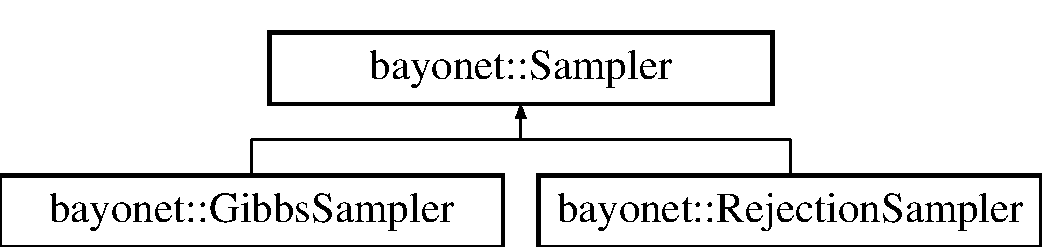
\includegraphics[height=2.000000cm]{classbayonet_1_1_sampler}
\end{center}
\end{figure}
\subsection*{Public Member Functions}
\begin{DoxyCompactItemize}
\item 
\hypertarget{classbayonet_1_1_sampler_a9fa53ea7b8204609e8bb2c02108445d5}{virtual std\-::vector$<$ unsigned int $>$ {\bfseries Return\-Sample} (\hyperlink{classbayonet_1_1_bayesnet}{Bayesnet})=0}\label{classbayonet_1_1_sampler_a9fa53ea7b8204609e8bb2c02108445d5}

\item 
\hypertarget{classbayonet_1_1_sampler_abf228d4fb18fb05d38e2394cce020007}{virtual std\-::vector\\*
$<$ std\-::vector$<$ unsigned int $>$ $>$ {\bfseries Accumulate\-Samples} (\hyperlink{classbayonet_1_1_bayesnet}{Bayesnet}, unsigned int cycles)=0}\label{classbayonet_1_1_sampler_abf228d4fb18fb05d38e2394cce020007}

\end{DoxyCompactItemize}
\subsection*{Protected Attributes}
\begin{DoxyCompactItemize}
\item 
\hypertarget{classbayonet_1_1_sampler_a87272da95dcc8028a13384931eda0d81}{std\-::vector$<$ unsigned int $>$ {\bfseries m\-Sample\-Vector}}\label{classbayonet_1_1_sampler_a87272da95dcc8028a13384931eda0d81}

\end{DoxyCompactItemize}


\subsection{Detailed Description}
A generic class that cannot be used for real. It is a framework for derived classes. 

The documentation for this class was generated from the following file\-:\begin{DoxyCompactItemize}
\item 
include/Sampler.\-h\end{DoxyCompactItemize}

%--- End generated contents ---

% Index
\newpage
\phantomsection
\addcontentsline{toc}{chapter}{Index}
\printindex

\end{document}
